\documentclass[twoside]{book}

% Packages required by doxygen
\usepackage{fixltx2e}
\usepackage{calc}
\usepackage{doxygen}
\usepackage[export]{adjustbox} % also loads graphicx
\usepackage{graphicx}
\usepackage[utf8]{inputenc}
\usepackage{makeidx}
\usepackage{multicol}
\usepackage{multirow}
\PassOptionsToPackage{warn}{textcomp}
\usepackage{textcomp}
\usepackage[nointegrals]{wasysym}
\usepackage[table]{xcolor}

% Font selection
\usepackage[T1]{fontenc}
\usepackage[scaled=.90]{helvet}
\usepackage{courier}
\usepackage{amssymb}
\usepackage{sectsty}
\renewcommand{\familydefault}{\sfdefault}
\allsectionsfont{%
  \fontseries{bc}\selectfont%
  \color{darkgray}%
}
\renewcommand{\DoxyLabelFont}{%
  \fontseries{bc}\selectfont%
  \color{darkgray}%
}
\newcommand{\+}{\discretionary{\mbox{\scriptsize$\hookleftarrow$}}{}{}}

% Page & text layout
\usepackage{geometry}
\geometry{%
  a4paper,%
  top=2.5cm,%
  bottom=2.5cm,%
  left=2.5cm,%
  right=2.5cm%
}
\tolerance=750
\hfuzz=15pt
\hbadness=750
\setlength{\emergencystretch}{15pt}
\setlength{\parindent}{0cm}
\setlength{\parskip}{3ex plus 2ex minus 2ex}
\makeatletter
\renewcommand{\paragraph}{%
  \@startsection{paragraph}{4}{0ex}{-1.0ex}{1.0ex}{%
    \normalfont\normalsize\bfseries\SS@parafont%
  }%
}
\renewcommand{\subparagraph}{%
  \@startsection{subparagraph}{5}{0ex}{-1.0ex}{1.0ex}{%
    \normalfont\normalsize\bfseries\SS@subparafont%
  }%
}
\makeatother

% Headers & footers
\usepackage{fancyhdr}
\pagestyle{fancyplain}
\fancyhead[LE]{\fancyplain{}{\bfseries\thepage}}
\fancyhead[CE]{\fancyplain{}{}}
\fancyhead[RE]{\fancyplain{}{\bfseries\leftmark}}
\fancyhead[LO]{\fancyplain{}{\bfseries\rightmark}}
\fancyhead[CO]{\fancyplain{}{}}
\fancyhead[RO]{\fancyplain{}{\bfseries\thepage}}
\fancyfoot[LE]{\fancyplain{}{}}
\fancyfoot[CE]{\fancyplain{}{}}
\fancyfoot[RE]{\fancyplain{}{\bfseries\scriptsize Generated by Doxygen }}
\fancyfoot[LO]{\fancyplain{}{\bfseries\scriptsize Generated by Doxygen }}
\fancyfoot[CO]{\fancyplain{}{}}
\fancyfoot[RO]{\fancyplain{}{}}
\renewcommand{\footrulewidth}{0.4pt}
\renewcommand{\chaptermark}[1]{%
  \markboth{#1}{}%
}
\renewcommand{\sectionmark}[1]{%
  \markright{\thesection\ #1}%
}

% Indices & bibliography
\usepackage{natbib}
\usepackage[titles]{tocloft}
\setcounter{tocdepth}{3}
\setcounter{secnumdepth}{5}
\makeindex

% Hyperlinks (required, but should be loaded last)
\usepackage{ifpdf}
\ifpdf
  \usepackage[pdftex,pagebackref=true]{hyperref}
\else
  \usepackage[ps2pdf,pagebackref=true]{hyperref}
\fi
\hypersetup{%
  colorlinks=true,%
  linkcolor=blue,%
  citecolor=blue,%
  unicode%
}

% Custom commands
\newcommand{\clearemptydoublepage}{%
  \newpage{\pagestyle{empty}\cleardoublepage}%
}

\usepackage{caption}
\captionsetup{labelsep=space,justification=centering,font={bf},singlelinecheck=off,skip=4pt,position=top}

%===== C O N T E N T S =====

\begin{document}

% Titlepage & ToC
\hypersetup{pageanchor=false,
             bookmarksnumbered=true,
             pdfencoding=unicode
            }
\pagenumbering{alph}
\begin{titlepage}
\vspace*{7cm}
\begin{center}%
{\Large Controller for multi mobile robot transport tasks }\\
\vspace*{1cm}
{\large Generated by Doxygen 1.8.13}\\
\end{center}
\end{titlepage}
\clearemptydoublepage
\pagenumbering{roman}
\tableofcontents
\clearemptydoublepage
\pagenumbering{arabic}
\hypersetup{pageanchor=true}

%--- Begin generated contents ---
\chapter{Formation Controller}
\label{md_README}
\Hypertarget{md_README}
This is the Implementation of the formation controller. It is implemented as Angle-\/\+Distance controller and as a kartesian tracking controller. An example of its configuration is given within the config directory with the controller.\+yaml file \section*{Leader and Follower}

Leader controller are master nodes (see master.\+h) while the follower robots are controlled by the slave node (see slave.\+h). 
\chapter{Module Index}
\section{Modules}
Here is a list of all modules\+:\begin{DoxyCompactList}
\item \contentsline{section}{Transport Controller}{\pageref{group__transport__controller}}{}
\begin{DoxyCompactList}
\item \contentsline{section}{Feed Forward Controller}{\pageref{group__group__feed__forward}}{}
\item \contentsline{section}{Robot Arm Controller}{\pageref{group__group__arm__controller}}{}
\end{DoxyCompactList}
\end{DoxyCompactList}

\chapter{Hierarchical Index}
\section{Class Hierarchy}
This inheritance list is sorted roughly, but not completely, alphabetically\+:\begin{DoxyCompactList}
\item \contentsline{section}{Orientation\+Feed\+Forward}{\pageref{classOrientationFeedForward}}{}
\begin{DoxyCompactList}
\item \contentsline{section}{Ros\+Orientation\+Feed\+Forward$<$ T $>$}{\pageref{classRosOrientationFeedForward}}{}
\end{DoxyCompactList}
\end{DoxyCompactList}

\chapter{Class Index}
\section{Class List}
Here are the classes, structs, unions and interfaces with brief descriptions\+:\begin{DoxyCompactList}
\item\contentsline{section}{\hyperlink{classConstrainedrigid__motion}{Constrainedrigid\+\_\+motion} }{\pageref{classConstrainedrigid__motion}}{}
\item\contentsline{section}{\hyperlink{classConstrainedrigid__motionRos}{Constrainedrigid\+\_\+motion\+Ros} }{\pageref{classConstrainedrigid__motionRos}}{}
\item\contentsline{section}{\hyperlink{classConstrainedrigid__motionTf}{Constrainedrigid\+\_\+motion\+Tf} }{\pageref{classConstrainedrigid__motionTf}}{}
\item\contentsline{section}{\hyperlink{classController}{Controller} }{\pageref{classController}}{}
\item\contentsline{section}{\hyperlink{structController_1_1ControlVector}{Controller\+::\+Control\+Vector} \\*Defines the controllers output }{\pageref{structController_1_1ControlVector}}{}
\item\contentsline{section}{\hyperlink{classInputAllocException}{Input\+Alloc\+Exception} }{\pageref{classInputAllocException}}{}
\item\contentsline{section}{\hyperlink{classInputBase}{Input\+Base} }{\pageref{classInputBase}}{}
\item\contentsline{section}{\hyperlink{classInputOdom}{Input\+Odom} }{\pageref{classInputOdom}}{}
\item\contentsline{section}{\hyperlink{classInputPoseOdom}{Input\+Pose\+Odom} }{\pageref{classInputPoseOdom}}{}
\item\contentsline{section}{\hyperlink{classInputPoseTwist}{Input\+Pose\+Twist} }{\pageref{classInputPoseTwist}}{}
\item\contentsline{section}{\hyperlink{classLyapunovController}{Lyapunov\+Controller} }{\pageref{classLyapunovController}}{}
\item\contentsline{section}{\hyperlink{structLyapunovController_1_1LyapunovParameter}{Lyapunov\+Controller\+::\+Lyapunov\+Parameter} \\*Holds the necessary parameters for the control law }{\pageref{structLyapunovController_1_1LyapunovParameter}}{}
\item\contentsline{section}{\hyperlink{classMsgOrientationFeedForward}{Msg\+Orientation\+Feed\+Forward$<$ T $>$} \\*A Ros implementation of the Orientation\+Feeed\+Forward class. It contains a ros Subscriber that listens to a specific message and uses the message data as input data for the feed forward control }{\pageref{classMsgOrientationFeedForward}}{}
\item\contentsline{section}{\hyperlink{classNecessaryParamException}{Necessary\+Param\+Exception} }{\pageref{classNecessaryParamException}}{}
\item\contentsline{section}{\hyperlink{classOrientationFeedForward}{Orientation\+Feed\+Forward} \\*A Orientation feed forward class. It uses a given orientation and calculates a robot arm pose that compansates the motion by the change of orientation (null space motion) }{\pageref{classOrientationFeedForward}}{}
\item\contentsline{section}{\hyperlink{classPassTroughController}{Pass\+Trough\+Controller} }{\pageref{classPassTroughController}}{}
\item\contentsline{section}{\hyperlink{classRosOrientationFeedForwardBase}{Ros\+Orientation\+Feed\+Forward\+Base} \\*A Orientation feed forward class. It implements parameter loading and initialisation for the Orientation Feed Forward class }{\pageref{classRosOrientationFeedForwardBase}}{}
\item\contentsline{section}{\hyperlink{structController_1_1State}{Controller\+::\+State} \\*Defines the state representations within the \hyperlink{classController}{Controller} }{\pageref{structController_1_1State}}{}
\item\contentsline{section}{\hyperlink{classTfOrientationFeedForward}{Tf\+Orientation\+Feed\+Forward} \\*A Tf implementation of the Orientation\+Feeed\+Forward class. It contains a tf listener that listens to a specific transformations and uses the data as input data for the feed forward control }{\pageref{classTfOrientationFeedForward}}{}
\end{DoxyCompactList}

\chapter{File Index}
\section{File List}
Here is a list of all documented files with brief descriptions\+:\begin{DoxyCompactList}
\item\contentsline{section}{include/multi\+\_\+robot\+\_\+controller/{\bfseries input\+\_\+alloc\+\_\+exception.\+hpp} }{\pageref{input__alloc__exception_8hpp}}{}
\item\contentsline{section}{include/multi\+\_\+robot\+\_\+controller/{\bfseries necessary\+\_\+param\+\_\+exeption.\+hpp} }{\pageref{necessary__param__exeption_8hpp}}{}
\item\contentsline{section}{include/multi\+\_\+robot\+\_\+controller/controller/{\bfseries controller.\+h} }{\pageref{controller_8h}}{}
\item\contentsline{section}{include/multi\+\_\+robot\+\_\+controller/controller/{\bfseries lyapunov\+\_\+controller.\+h} }{\pageref{lyapunov__controller_8h}}{}
\item\contentsline{section}{include/multi\+\_\+robot\+\_\+controller/controller/{\bfseries pass\+\_\+through\+\_\+controller.\+hpp} }{\pageref{pass__through__controller_8hpp}}{}
\item\contentsline{section}{include/multi\+\_\+robot\+\_\+controller/feed\+\_\+forward/\hyperlink{msg__conversion_8hpp}{msg\+\_\+conversion.\+hpp} }{\pageref{msg__conversion_8hpp}}{}
\item\contentsline{section}{include/multi\+\_\+robot\+\_\+controller/feed\+\_\+forward/{\bfseries msg\+\_\+orientation\+\_\+feed\+\_\+forward.\+h} }{\pageref{msg__orientation__feed__forward_8h}}{}
\item\contentsline{section}{include/multi\+\_\+robot\+\_\+controller/feed\+\_\+forward/{\bfseries orientation\+\_\+feed\+\_\+forward.\+h} }{\pageref{orientation__feed__forward_8h}}{}
\item\contentsline{section}{include/multi\+\_\+robot\+\_\+controller/feed\+\_\+forward/{\bfseries ros\+\_\+orientation\+\_\+feed\+\_\+forward\+\_\+base.\+h} }{\pageref{ros__orientation__feed__forward__base_8h}}{}
\item\contentsline{section}{include/multi\+\_\+robot\+\_\+controller/feed\+\_\+forward/{\bfseries tf\+\_\+orientation\+\_\+feed\+\_\+forward.\+h} }{\pageref{tf__orientation__feed__forward_8h}}{}
\item\contentsline{section}{include/multi\+\_\+robot\+\_\+controller/input/{\bfseries input\+\_\+base.\+hpp} }{\pageref{input__base_8hpp}}{}
\item\contentsline{section}{include/multi\+\_\+robot\+\_\+controller/input/{\bfseries input\+\_\+odom.\+hpp} }{\pageref{input__odom_8hpp}}{}
\item\contentsline{section}{include/multi\+\_\+robot\+\_\+controller/input/{\bfseries input\+\_\+pose\+\_\+odom.\+hpp} }{\pageref{input__pose__odom_8hpp}}{}
\item\contentsline{section}{include/multi\+\_\+robot\+\_\+controller/input/{\bfseries input\+\_\+pose\+\_\+twist.\+hpp} }{\pageref{input__pose__twist_8hpp}}{}
\item\contentsline{section}{include/multi\+\_\+robot\+\_\+controller/input/{\bfseries input\+\_\+types.\+hpp} }{\pageref{input__types_8hpp}}{}
\item\contentsline{section}{include/multi\+\_\+robot\+\_\+controller/rigid\+\_\+motion/{\bfseries constrained\+\_\+rigid\+\_\+motion.\+h} }{\pageref{constrained__rigid__motion_8h}}{}
\item\contentsline{section}{include/multi\+\_\+robot\+\_\+controller/rigid\+\_\+motion/{\bfseries constrained\+\_\+rigid\+\_\+motion\+\_\+ros.\+h} }{\pageref{constrained__rigid__motion__ros_8h}}{}
\item\contentsline{section}{include/multi\+\_\+robot\+\_\+controller/rigid\+\_\+motion/{\bfseries constrained\+\_\+rigid\+\_\+motion\+\_\+tf.\+h} }{\pageref{constrained__rigid__motion__tf_8h}}{}
\end{DoxyCompactList}

\chapter{Module Documentation}
\hypertarget{group__MultiRobotController}{}\section{Multi\+Robot\+Controller}
\label{group__MultiRobotController}\index{Multi\+Robot\+Controller@{Multi\+Robot\+Controller}}
\subsection*{Classes}
\begin{DoxyCompactItemize}
\item 
class \hyperlink{classInputAllocException}{Input\+Alloc\+Exception}
\item 
class \hyperlink{classNecessaryParamException}{Necessary\+Param\+Exception}
\end{DoxyCompactItemize}
\subsection*{Functions}
\begin{DoxyCompactItemize}
\item 
void \hyperlink{group__MultiRobotController_ga465b07e16106af072ed5315010fa876c}{convert\+Msg} (Eigen\+::\+Quaterniond \&quat, std\+\_\+msgs\+::\+Float64 \&msg)
\begin{DoxyCompactList}\small\item\em Convert an float64 z-\/axis angle to an eigen quaternion. \end{DoxyCompactList}\item 
void \hyperlink{group__MultiRobotController_gad42169e0be94216cd31a8a360a848155}{convert\+Msg} (Eigen\+::\+Quaterniond \&quat, geometry\+\_\+msgs\+::\+Transform \&msg)
\begin{DoxyCompactList}\small\item\em Convert Orientation of a Transform geometry message to an eigen quaternion. \end{DoxyCompactList}\item 
void \hyperlink{group__MultiRobotController_ga34987bf2293cc8aa5fac7ac60e6510ef}{convert\+Msg} (Eigen\+::\+Quaterniond \&quat, geometry\+\_\+msgs\+::\+Transform\+Stamped \&msg)
\begin{DoxyCompactList}\small\item\em Convert an Stamped\+Transform geometry message to an eigen quaternion. \end{DoxyCompactList}\item 
void \hyperlink{group__MultiRobotController_gadc07db93efb76fd809b67b74dd13b939}{convert\+Msg} (Eigen\+::\+Quaterniond \&quat, geometry\+\_\+msgs\+::\+Pose \&msg)
\begin{DoxyCompactList}\small\item\em Convert an Pose geometry message to an eigen quaternion. \end{DoxyCompactList}\item 
void \hyperlink{group__MultiRobotController_ga8257db2bb94ec53eadfe87d04b38cc0b}{convert\+Msg} (Eigen\+::\+Quaterniond \&quat, geometry\+\_\+msgs\+::\+Pose\+Stamped \&msg)
\begin{DoxyCompactList}\small\item\em Convert an stamped pose geometry message to an eigen quaternion. \end{DoxyCompactList}\item 
void \hyperlink{group__MultiRobotController_gafde5764b46f0189c2aea14ed57434708}{convert\+Msg} (Eigen\+::\+Matrix$<$ double, 7, 1 $>$ \&pose, geometry\+\_\+msgs\+::\+Pose \&msg)
\begin{DoxyCompactList}\small\item\em Convert an pose geometry message to an Eigen pose vector (x, y, z, w, x, y, z) \end{DoxyCompactList}\item 
void \hyperlink{group__MultiRobotController_ga9e842115a5f448ab0e3ba9fea93d5179}{convert\+Msg} (Eigen\+::\+Matrix$<$ double, 7, 1 $>$ \&pose, geometry\+\_\+msgs\+::\+Pose\+Stamped \&msg)
\begin{DoxyCompactList}\small\item\em Convert an stamepd pose geometry message to an Eigen pose vector (x, y, z, w, x, y, z) \end{DoxyCompactList}\item 
void \hyperlink{group__MultiRobotController_ga7beb50c98e49263d05b3b819be58d76c}{convert\+Msg} (geometry\+\_\+msgs\+::\+Pose \&msg, Eigen\+::\+Matrix$<$ double, 7, 1 $>$ \&pose)
\begin{DoxyCompactList}\small\item\em Convert an Eigen pose vector (x, y, z, w, x, y, z) to a pose geometry message. \end{DoxyCompactList}\item 
void \hyperlink{group__MultiRobotController_gaf1628de186f2d90b064f8c8b36beef53}{convert\+Msg} (geometry\+\_\+msgs\+::\+Pose\+Stamped \&msg, Eigen\+::\+Matrix$<$ double, 7, 1 $>$ \&pose)
\begin{DoxyCompactList}\small\item\em Convert an Eigen pose vector (x, y, z, w, x, y, z) to a stamepd pose geometry message. \end{DoxyCompactList}\item 
void \hyperlink{group__MultiRobotController_ga45b2bbef58d2c60ff8eeb77d221f2ab7}{convert\+Msg} (geometry\+\_\+msgs\+::\+Pose \&pose, geometry\+\_\+msgs\+::\+Transform \&transform)
\begin{DoxyCompactList}\small\item\em Convert an Eigen pose vector (x, y, z, w, x, y, z) to a transform geometry message. \end{DoxyCompactList}\item 
void \hyperlink{group__MultiRobotController_gaf99f4d3d714176ee5a3d235ffabb7d3f}{convert\+Msg} (geometry\+\_\+msgs\+::\+Pose\+Stamped \&pose, geometry\+\_\+msgs\+::\+Transform\+Stamped \&transform\+Stamped)
\begin{DoxyCompactList}\small\item\em Convert a stamped transform geometry message to a stamped pose geometry message. \end{DoxyCompactList}\item 
void \hyperlink{group__MultiRobotController_ga21e894dfe1e1216355db06776a630b09}{convert\+Msg} (Eigen\+::\+Matrix$<$ double, 7, 1 $>$ \&pose, geometry\+\_\+msgs\+::\+Transform\+Stamped \&transform\+Stamped)
\begin{DoxyCompactList}\small\item\em Convert a stamped transform geometry message to a eigen pose vector. \end{DoxyCompactList}\item 
void \hyperlink{group__MultiRobotController_ga27bedbf17c4aa6e228239ef1f1009e2b}{convert\+Msg} (geometry\+\_\+msgs\+::\+Transform \&transform, geometry\+\_\+msgs\+::\+Pose \&pose)
\begin{DoxyCompactList}\small\item\em Convert a geometry pos messag to a geometry transfomr message. \end{DoxyCompactList}\item 
void \hyperlink{group__MultiRobotController_ga83f417b8e164774e4926508549543498}{convert\+Msg} (geometry\+\_\+msgs\+::\+Transform\+Stamped \&transform, geometry\+\_\+msgs\+::\+Pose\+Stamped \&pose)
\begin{DoxyCompactList}\small\item\em Convert a geometry stamped pose message to a stamped transform geometry message. \end{DoxyCompactList}\item 
\mbox{\Hypertarget{group__MultiRobotController_gaa948b5d25acee95c1d39f1e1276304b8}\label{group__MultiRobotController_gaa948b5d25acee95c1d39f1e1276304b8}} 
const char $\ast$ {\bfseries Input\+Alloc\+Exception\+::what} () const  throw ()
\item 
\mbox{\Hypertarget{group__MultiRobotController_ga7c6066c92d689e7946e49425c2efef62}\label{group__MultiRobotController_ga7c6066c92d689e7946e49425c2efef62}} 
{\bfseries Necessary\+Param\+Exception\+::\+Necessary\+Param\+Exception} (std\+::string param\+\_\+name\+\_\+resolved)
\end{DoxyCompactItemize}


\subsection{Detailed Description}


\subsection{Function Documentation}
\mbox{\Hypertarget{group__MultiRobotController_ga465b07e16106af072ed5315010fa876c}\label{group__MultiRobotController_ga465b07e16106af072ed5315010fa876c}} 
\index{Multi\+Robot\+Controller@{Multi\+Robot\+Controller}!convert\+Msg@{convert\+Msg}}
\index{convert\+Msg@{convert\+Msg}!Multi\+Robot\+Controller@{Multi\+Robot\+Controller}}
\subsubsection{\texorpdfstring{convert\+Msg()}{convertMsg()}\hspace{0.1cm}{\footnotesize\ttfamily [1/14]}}
{\footnotesize\ttfamily void convert\+Msg (\begin{DoxyParamCaption}\item[{Eigen\+::\+Quaterniond \&}]{quat,  }\item[{std\+\_\+msgs\+::\+Float64 \&}]{msg }\end{DoxyParamCaption})\hspace{0.3cm}{\ttfamily [inline]}}


\begin{DoxyParams}{Parameters}
{\em msg} & Float64 ros message with z-\/axis angle \\
\hline
{\em quat} & Eigen quaterniond the quaternion is stored in \\
\hline
\end{DoxyParams}
\mbox{\Hypertarget{group__MultiRobotController_gad42169e0be94216cd31a8a360a848155}\label{group__MultiRobotController_gad42169e0be94216cd31a8a360a848155}} 
\index{Multi\+Robot\+Controller@{Multi\+Robot\+Controller}!convert\+Msg@{convert\+Msg}}
\index{convert\+Msg@{convert\+Msg}!Multi\+Robot\+Controller@{Multi\+Robot\+Controller}}
\subsubsection{\texorpdfstring{convert\+Msg()}{convertMsg()}\hspace{0.1cm}{\footnotesize\ttfamily [2/14]}}
{\footnotesize\ttfamily void convert\+Msg (\begin{DoxyParamCaption}\item[{Eigen\+::\+Quaterniond \&}]{quat,  }\item[{geometry\+\_\+msgs\+::\+Transform \&}]{msg }\end{DoxyParamCaption})\hspace{0.3cm}{\ttfamily [inline]}}


\begin{DoxyParams}{Parameters}
{\em msg} & Message that holds the transform \\
\hline
{\em quat} & Quaternion the eigen quaternion is stored in \\
\hline
\end{DoxyParams}
\mbox{\Hypertarget{group__MultiRobotController_ga34987bf2293cc8aa5fac7ac60e6510ef}\label{group__MultiRobotController_ga34987bf2293cc8aa5fac7ac60e6510ef}} 
\index{Multi\+Robot\+Controller@{Multi\+Robot\+Controller}!convert\+Msg@{convert\+Msg}}
\index{convert\+Msg@{convert\+Msg}!Multi\+Robot\+Controller@{Multi\+Robot\+Controller}}
\subsubsection{\texorpdfstring{convert\+Msg()}{convertMsg()}\hspace{0.1cm}{\footnotesize\ttfamily [3/14]}}
{\footnotesize\ttfamily void convert\+Msg (\begin{DoxyParamCaption}\item[{Eigen\+::\+Quaterniond \&}]{quat,  }\item[{geometry\+\_\+msgs\+::\+Transform\+Stamped \&}]{msg }\end{DoxyParamCaption})\hspace{0.3cm}{\ttfamily [inline]}}


\begin{DoxyParams}{Parameters}
{\em msg} & Message that holds the stamped transform \\
\hline
{\em quat} & Quternion the eigen quaternion is stored in \\
\hline
\end{DoxyParams}
\mbox{\Hypertarget{group__MultiRobotController_gadc07db93efb76fd809b67b74dd13b939}\label{group__MultiRobotController_gadc07db93efb76fd809b67b74dd13b939}} 
\index{Multi\+Robot\+Controller@{Multi\+Robot\+Controller}!convert\+Msg@{convert\+Msg}}
\index{convert\+Msg@{convert\+Msg}!Multi\+Robot\+Controller@{Multi\+Robot\+Controller}}
\subsubsection{\texorpdfstring{convert\+Msg()}{convertMsg()}\hspace{0.1cm}{\footnotesize\ttfamily [4/14]}}
{\footnotesize\ttfamily void convert\+Msg (\begin{DoxyParamCaption}\item[{Eigen\+::\+Quaterniond \&}]{quat,  }\item[{geometry\+\_\+msgs\+::\+Pose \&}]{msg }\end{DoxyParamCaption})\hspace{0.3cm}{\ttfamily [inline]}}


\begin{DoxyParams}{Parameters}
{\em msg} & Message that holds the pose \\
\hline
{\em quat} & Quternion the eigen quaternion is stored in \\
\hline
\end{DoxyParams}
\mbox{\Hypertarget{group__MultiRobotController_ga8257db2bb94ec53eadfe87d04b38cc0b}\label{group__MultiRobotController_ga8257db2bb94ec53eadfe87d04b38cc0b}} 
\index{Multi\+Robot\+Controller@{Multi\+Robot\+Controller}!convert\+Msg@{convert\+Msg}}
\index{convert\+Msg@{convert\+Msg}!Multi\+Robot\+Controller@{Multi\+Robot\+Controller}}
\subsubsection{\texorpdfstring{convert\+Msg()}{convertMsg()}\hspace{0.1cm}{\footnotesize\ttfamily [5/14]}}
{\footnotesize\ttfamily void convert\+Msg (\begin{DoxyParamCaption}\item[{Eigen\+::\+Quaterniond \&}]{quat,  }\item[{geometry\+\_\+msgs\+::\+Pose\+Stamped \&}]{msg }\end{DoxyParamCaption})\hspace{0.3cm}{\ttfamily [inline]}}


\begin{DoxyParams}{Parameters}
{\em msg} & Message that holds the stamped pose \\
\hline
{\em quat} & Quternion the eigen quaternion is stored in \\
\hline
\end{DoxyParams}
\mbox{\Hypertarget{group__MultiRobotController_gafde5764b46f0189c2aea14ed57434708}\label{group__MultiRobotController_gafde5764b46f0189c2aea14ed57434708}} 
\index{Multi\+Robot\+Controller@{Multi\+Robot\+Controller}!convert\+Msg@{convert\+Msg}}
\index{convert\+Msg@{convert\+Msg}!Multi\+Robot\+Controller@{Multi\+Robot\+Controller}}
\subsubsection{\texorpdfstring{convert\+Msg()}{convertMsg()}\hspace{0.1cm}{\footnotesize\ttfamily [6/14]}}
{\footnotesize\ttfamily void convert\+Msg (\begin{DoxyParamCaption}\item[{Eigen\+::\+Matrix$<$ double, 7, 1 $>$ \&}]{pose,  }\item[{geometry\+\_\+msgs\+::\+Pose \&}]{msg }\end{DoxyParamCaption})\hspace{0.3cm}{\ttfamily [inline]}}


\begin{DoxyParams}{Parameters}
{\em msg} & Message that holds the pose \\
\hline
{\em pose} & Matrix (Vector) the eigen pose vector is stored in \\
\hline
\end{DoxyParams}
\mbox{\Hypertarget{group__MultiRobotController_ga9e842115a5f448ab0e3ba9fea93d5179}\label{group__MultiRobotController_ga9e842115a5f448ab0e3ba9fea93d5179}} 
\index{Multi\+Robot\+Controller@{Multi\+Robot\+Controller}!convert\+Msg@{convert\+Msg}}
\index{convert\+Msg@{convert\+Msg}!Multi\+Robot\+Controller@{Multi\+Robot\+Controller}}
\subsubsection{\texorpdfstring{convert\+Msg()}{convertMsg()}\hspace{0.1cm}{\footnotesize\ttfamily [7/14]}}
{\footnotesize\ttfamily void convert\+Msg (\begin{DoxyParamCaption}\item[{Eigen\+::\+Matrix$<$ double, 7, 1 $>$ \&}]{pose,  }\item[{geometry\+\_\+msgs\+::\+Pose\+Stamped \&}]{msg }\end{DoxyParamCaption})\hspace{0.3cm}{\ttfamily [inline]}}


\begin{DoxyParams}{Parameters}
{\em msg} & Message that holds the pose \\
\hline
{\em pose} & Matrix (Vector) the eigen pose vector is stored in \\
\hline
\end{DoxyParams}
\mbox{\Hypertarget{group__MultiRobotController_ga7beb50c98e49263d05b3b819be58d76c}\label{group__MultiRobotController_ga7beb50c98e49263d05b3b819be58d76c}} 
\index{Multi\+Robot\+Controller@{Multi\+Robot\+Controller}!convert\+Msg@{convert\+Msg}}
\index{convert\+Msg@{convert\+Msg}!Multi\+Robot\+Controller@{Multi\+Robot\+Controller}}
\subsubsection{\texorpdfstring{convert\+Msg()}{convertMsg()}\hspace{0.1cm}{\footnotesize\ttfamily [8/14]}}
{\footnotesize\ttfamily void convert\+Msg (\begin{DoxyParamCaption}\item[{geometry\+\_\+msgs\+::\+Pose \&}]{msg,  }\item[{Eigen\+::\+Matrix$<$ double, 7, 1 $>$ \&}]{pose }\end{DoxyParamCaption})\hspace{0.3cm}{\ttfamily [inline]}}


\begin{DoxyParams}{Parameters}
{\em msg} & Message that the pose is stored in \\
\hline
{\em pose} & Matrix (Vector) that holds the pose \\
\hline
\end{DoxyParams}
\mbox{\Hypertarget{group__MultiRobotController_gaf1628de186f2d90b064f8c8b36beef53}\label{group__MultiRobotController_gaf1628de186f2d90b064f8c8b36beef53}} 
\index{Multi\+Robot\+Controller@{Multi\+Robot\+Controller}!convert\+Msg@{convert\+Msg}}
\index{convert\+Msg@{convert\+Msg}!Multi\+Robot\+Controller@{Multi\+Robot\+Controller}}
\subsubsection{\texorpdfstring{convert\+Msg()}{convertMsg()}\hspace{0.1cm}{\footnotesize\ttfamily [9/14]}}
{\footnotesize\ttfamily void convert\+Msg (\begin{DoxyParamCaption}\item[{geometry\+\_\+msgs\+::\+Pose\+Stamped \&}]{msg,  }\item[{Eigen\+::\+Matrix$<$ double, 7, 1 $>$ \&}]{pose }\end{DoxyParamCaption})\hspace{0.3cm}{\ttfamily [inline]}}


\begin{DoxyParams}{Parameters}
{\em msg} & Message that the pose is stored in \\
\hline
{\em pose} & Matrix (Vector) that holds the pose \\
\hline
\end{DoxyParams}
\mbox{\Hypertarget{group__MultiRobotController_ga45b2bbef58d2c60ff8eeb77d221f2ab7}\label{group__MultiRobotController_ga45b2bbef58d2c60ff8eeb77d221f2ab7}} 
\index{Multi\+Robot\+Controller@{Multi\+Robot\+Controller}!convert\+Msg@{convert\+Msg}}
\index{convert\+Msg@{convert\+Msg}!Multi\+Robot\+Controller@{Multi\+Robot\+Controller}}
\subsubsection{\texorpdfstring{convert\+Msg()}{convertMsg()}\hspace{0.1cm}{\footnotesize\ttfamily [10/14]}}
{\footnotesize\ttfamily void convert\+Msg (\begin{DoxyParamCaption}\item[{geometry\+\_\+msgs\+::\+Pose \&}]{pose,  }\item[{geometry\+\_\+msgs\+::\+Transform \&}]{transform }\end{DoxyParamCaption})\hspace{0.3cm}{\ttfamily [inline]}}


\begin{DoxyParams}{Parameters}
{\em msg} & Message that the pose is stored in \\
\hline
{\em pose} & Matrix (Vector) that holds the pose \\
\hline
\end{DoxyParams}
\mbox{\Hypertarget{group__MultiRobotController_gaf99f4d3d714176ee5a3d235ffabb7d3f}\label{group__MultiRobotController_gaf99f4d3d714176ee5a3d235ffabb7d3f}} 
\index{Multi\+Robot\+Controller@{Multi\+Robot\+Controller}!convert\+Msg@{convert\+Msg}}
\index{convert\+Msg@{convert\+Msg}!Multi\+Robot\+Controller@{Multi\+Robot\+Controller}}
\subsubsection{\texorpdfstring{convert\+Msg()}{convertMsg()}\hspace{0.1cm}{\footnotesize\ttfamily [11/14]}}
{\footnotesize\ttfamily void convert\+Msg (\begin{DoxyParamCaption}\item[{geometry\+\_\+msgs\+::\+Pose\+Stamped \&}]{pose,  }\item[{geometry\+\_\+msgs\+::\+Transform\+Stamped \&}]{transform\+Stamped }\end{DoxyParamCaption})\hspace{0.3cm}{\ttfamily [inline]}}


\begin{DoxyParams}{Parameters}
{\em pose} & Stamped pose the pose is stored in \\
\hline
{\em transform\+Stamped} & The geometry msgs that holds the transform \\
\hline
\end{DoxyParams}
\mbox{\Hypertarget{group__MultiRobotController_ga21e894dfe1e1216355db06776a630b09}\label{group__MultiRobotController_ga21e894dfe1e1216355db06776a630b09}} 
\index{Multi\+Robot\+Controller@{Multi\+Robot\+Controller}!convert\+Msg@{convert\+Msg}}
\index{convert\+Msg@{convert\+Msg}!Multi\+Robot\+Controller@{Multi\+Robot\+Controller}}
\subsubsection{\texorpdfstring{convert\+Msg()}{convertMsg()}\hspace{0.1cm}{\footnotesize\ttfamily [12/14]}}
{\footnotesize\ttfamily void convert\+Msg (\begin{DoxyParamCaption}\item[{Eigen\+::\+Matrix$<$ double, 7, 1 $>$ \&}]{pose,  }\item[{geometry\+\_\+msgs\+::\+Transform\+Stamped \&}]{transform\+Stamped }\end{DoxyParamCaption})\hspace{0.3cm}{\ttfamily [inline]}}


\begin{DoxyParams}{Parameters}
{\em pose} & Pose Vector the pose is stored in \\
\hline
{\em transform\+Stamped} & The geometry msgs that holds the transform \\
\hline
\end{DoxyParams}
\mbox{\Hypertarget{group__MultiRobotController_ga27bedbf17c4aa6e228239ef1f1009e2b}\label{group__MultiRobotController_ga27bedbf17c4aa6e228239ef1f1009e2b}} 
\index{Multi\+Robot\+Controller@{Multi\+Robot\+Controller}!convert\+Msg@{convert\+Msg}}
\index{convert\+Msg@{convert\+Msg}!Multi\+Robot\+Controller@{Multi\+Robot\+Controller}}
\subsubsection{\texorpdfstring{convert\+Msg()}{convertMsg()}\hspace{0.1cm}{\footnotesize\ttfamily [13/14]}}
{\footnotesize\ttfamily void convert\+Msg (\begin{DoxyParamCaption}\item[{geometry\+\_\+msgs\+::\+Transform \&}]{transform,  }\item[{geometry\+\_\+msgs\+::\+Pose \&}]{pose }\end{DoxyParamCaption})\hspace{0.3cm}{\ttfamily [inline]}}


\begin{DoxyParams}{Parameters}
{\em transform} & Message the transform is stored in \\
\hline
{\em pose} & Message that holds the pose \\
\hline
\end{DoxyParams}
\mbox{\Hypertarget{group__MultiRobotController_ga83f417b8e164774e4926508549543498}\label{group__MultiRobotController_ga83f417b8e164774e4926508549543498}} 
\index{Multi\+Robot\+Controller@{Multi\+Robot\+Controller}!convert\+Msg@{convert\+Msg}}
\index{convert\+Msg@{convert\+Msg}!Multi\+Robot\+Controller@{Multi\+Robot\+Controller}}
\subsubsection{\texorpdfstring{convert\+Msg()}{convertMsg()}\hspace{0.1cm}{\footnotesize\ttfamily [14/14]}}
{\footnotesize\ttfamily void convert\+Msg (\begin{DoxyParamCaption}\item[{geometry\+\_\+msgs\+::\+Transform\+Stamped \&}]{transform,  }\item[{geometry\+\_\+msgs\+::\+Pose\+Stamped \&}]{pose }\end{DoxyParamCaption})\hspace{0.3cm}{\ttfamily [inline]}}


\begin{DoxyParams}{Parameters}
{\em transform} & Message the stamped transform is stored in \\
\hline
{\em pose} & Message that holds the pose \\
\hline
\end{DoxyParams}

\hypertarget{group__FeedForward}{}\section{Feed\+Forward}
\label{group__FeedForward}\index{Feed\+Forward@{Feed\+Forward}}
\subsection*{Classes}
\begin{DoxyCompactItemize}
\item 
class \hyperlink{classMsgOrientationFeedForward}{Msg\+Orientation\+Feed\+Forward$<$ T $>$}
\begin{DoxyCompactList}\small\item\em A Ros implementation of the Orientation\+Feeed\+Forward class. It contains a ros Subscriber that listens to a specific message and uses the message data as input data for the feed forward control. \end{DoxyCompactList}\item 
class \hyperlink{classTfOrientationFeedForward}{Tf\+Orientation\+Feed\+Forward}
\begin{DoxyCompactList}\small\item\em A Tf implementation of the Orientation\+Feeed\+Forward class. It contains a tf listener that listens to a specific transformations and uses the data as input data for the feed forward control. \end{DoxyCompactList}\end{DoxyCompactItemize}


\subsection{Detailed Description}

\hypertarget{group__Input}{}\section{Input}
\label{group__Input}\index{Input@{Input}}
\subsection*{Classes}
\begin{DoxyCompactItemize}
\item 
class \hyperlink{classInputBase}{Input\+Base}
\item 
class \hyperlink{classInputOdom}{Input\+Odom}
\item 
class \hyperlink{classInputPoseOdom}{Input\+Pose\+Odom}
\item 
class \hyperlink{classInputPoseTwist}{Input\+Pose\+Twist}
\item 
class \hyperlink{classInputPoseTwistLocal}{Input\+Pose\+Twist\+Local}
\end{DoxyCompactItemize}
\subsection*{Enumerations}
\begin{DoxyCompactItemize}
\item 
\mbox{\Hypertarget{group__Input_gaf4789bd72e7b14daae9ed61dbc059261}\label{group__Input_gaf4789bd72e7b14daae9ed61dbc059261}} 
enum {\bfseries Input\+Types} \{ \newline
{\bfseries P\+O\+S\+E\+\_\+\+O\+D\+OM} =0, 
{\bfseries S\+I\+N\+G\+L\+E\+\_\+\+O\+D\+OM} =1, 
{\bfseries P\+O\+S\+E\+\_\+\+T\+W\+I\+ST} =2, 
{\bfseries P\+O\+S\+E\+\_\+\+T\+W\+I\+S\+T\+\_\+\+L\+O\+C\+AL} =3, 
\newline
{\bfseries N\+O\+\_\+\+T\+Y\+PE}
 \}
\end{DoxyCompactItemize}
\subsection*{Functions}
\begin{DoxyCompactItemize}
\item 
\mbox{\Hypertarget{group__Input_gae49ba3ba26afd0315dc99f055b8d2f43}\label{group__Input_gae49ba3ba26afd0315dc99f055b8d2f43}} 
{\bfseries Input\+Base\+::\+Input\+Base} (ros\+::\+Node\+Handle \&nh)
\item 
\mbox{\Hypertarget{group__Input_gac7dcd07984459ebc0c23436a4170bfbc}\label{group__Input_gac7dcd07984459ebc0c23436a4170bfbc}} 
tf\+::\+Pose {\bfseries Input\+Base\+::get\+Pose} ()
\item 
\mbox{\Hypertarget{group__Input_gaf7b759985fd0b5d278050864382b2c57}\label{group__Input_gaf7b759985fd0b5d278050864382b2c57}} 
tf\+::\+Vector3 {\bfseries Input\+Base\+::get\+Lin\+Vel} ()
\item 
\mbox{\Hypertarget{group__Input_ga89ed5c155c3326ca3b266b9ae76b9f94}\label{group__Input_ga89ed5c155c3326ca3b266b9ae76b9f94}} 
tf\+::\+Vector3 {\bfseries Input\+Base\+::get\+Ang\+Vel} ()
\item 
\mbox{\Hypertarget{group__Input_ga3218880f2d8bf2d992875815d9264074}\label{group__Input_ga3218880f2d8bf2d992875815d9264074}} 
ros\+::\+Time {\bfseries Input\+Base\+::get\+Time} ()
\item 
\mbox{\Hypertarget{group__Input_gafa9f4394ddd1e7d309fd6cafcd966357}\label{group__Input_gafa9f4394ddd1e7d309fd6cafcd966357}} 
void {\bfseries Input\+Base\+::check\+Values} ()
\item 
\mbox{\Hypertarget{group__Input_gaf881b8cce924ac7c6ada67a779696606}\label{group__Input_gaf881b8cce924ac7c6ada67a779696606}} 
{\bfseries Input\+Odom\+::\+Input\+Odom} (ros\+::\+Node\+Handle \&nh, std\+::string topic\+\_\+name)
\item 
\mbox{\Hypertarget{group__Input_gad3ef3816f437f8cd96c6fee8c7b1ba2a}\label{group__Input_gad3ef3816f437f8cd96c6fee8c7b1ba2a}} 
{\bfseries Input\+Odom\+::\+Input\+Odom} (ros\+::\+Node\+Handle \&nh)
\item 
\mbox{\Hypertarget{group__Input_ga8c3c565c212707fbe1d33a412170465d}\label{group__Input_ga8c3c565c212707fbe1d33a412170465d}} 
{\bfseries Input\+Odom\+::\+Input\+Odom} (ros\+::\+Node\+Handle \&nh, ros\+::\+Node\+Handle \&param\+\_\+nh)
\item 
\mbox{\Hypertarget{group__Input_gad2de7e036d10a05678ac2489a97f84db}\label{group__Input_gad2de7e036d10a05678ac2489a97f84db}} 
{\bfseries Input\+Pose\+Odom\+::\+Input\+Pose\+Odom} (ros\+::\+Node\+Handle \&nh, std\+::string topic\+\_\+name\+\_\+pose, std\+::string topic\+\_\+name\+\_\+odom)
\item 
\mbox{\Hypertarget{group__Input_gaf65f517b5791a223d38d9e08a4c318b5}\label{group__Input_gaf65f517b5791a223d38d9e08a4c318b5}} 
{\bfseries Input\+Pose\+Odom\+::\+Input\+Pose\+Odom} (ros\+::\+Node\+Handle \&nh)
\item 
\mbox{\Hypertarget{group__Input_ga178d03771536f57e834e122485d3e73e}\label{group__Input_ga178d03771536f57e834e122485d3e73e}} 
{\bfseries Input\+Pose\+Odom\+::\+Input\+Pose\+Odom} (ros\+::\+Node\+Handle \&nh, ros\+::\+Node\+Handle \&nh\+\_\+param)
\item 
\mbox{\Hypertarget{group__Input_ga81300e68b133bd3df8fabf4d2ea7e4b2}\label{group__Input_ga81300e68b133bd3df8fabf4d2ea7e4b2}} 
{\bfseries Input\+Pose\+Twist\+::\+Input\+Pose\+Twist} (ros\+::\+Node\+Handle \&nh, std\+::string topic\+\_\+name\+\_\+pose, std\+::string topic\+\_\+name\+\_\+twist)
\item 
\mbox{\Hypertarget{group__Input_ga118fe4becb20679b5c950827b3b4b449}\label{group__Input_ga118fe4becb20679b5c950827b3b4b449}} 
{\bfseries Input\+Pose\+Twist\+::\+Input\+Pose\+Twist} (ros\+::\+Node\+Handle \&nh)
\item 
\mbox{\Hypertarget{group__Input_ga0e8c731f5d891db652aabe3d0b6bd92a}\label{group__Input_ga0e8c731f5d891db652aabe3d0b6bd92a}} 
{\bfseries Input\+Pose\+Twist\+::\+Input\+Pose\+Twist} (ros\+::\+Node\+Handle \&nh, ros\+::\+Node\+Handle \&nh\+\_\+param)
\item 
\mbox{\Hypertarget{group__Input_ga613203eb75ab62bb69d211bb41ff09ce}\label{group__Input_ga613203eb75ab62bb69d211bb41ff09ce}} 
{\bfseries Input\+Pose\+Twist\+Local\+::\+Input\+Pose\+Twist\+Local} (ros\+::\+Node\+Handle \&nh, std\+::string topic\+\_\+name\+\_\+pose, std\+::string topic\+\_\+name\+\_\+twist)
\item 
\mbox{\Hypertarget{group__Input_ga62a12e3ef3c56dfa955224d66cd21c17}\label{group__Input_ga62a12e3ef3c56dfa955224d66cd21c17}} 
{\bfseries Input\+Pose\+Twist\+Local\+::\+Input\+Pose\+Twist\+Local} (ros\+::\+Node\+Handle \&nh)
\item 
\mbox{\Hypertarget{group__Input_gac6c272dad9e420c67549b152d4c2581c}\label{group__Input_gac6c272dad9e420c67549b152d4c2581c}} 
{\bfseries Input\+Pose\+Twist\+Local\+::\+Input\+Pose\+Twist\+Local} (ros\+::\+Node\+Handle \&nh, ros\+::\+Node\+Handle \&nh\+\_\+param)
\end{DoxyCompactItemize}
\subsection*{Variables}
\begin{DoxyCompactItemize}
\item 
\mbox{\Hypertarget{group__Input_ga0a51906c129d50a4cb72c9490366f908}\label{group__Input_ga0a51906c129d50a4cb72c9490366f908}} 
ros\+::\+Node\+Handle {\bfseries Input\+Base\+::nh\+\_\+}
\item 
\mbox{\Hypertarget{group__Input_ga6642dbf660c3920565cbe03362cef669}\label{group__Input_ga6642dbf660c3920565cbe03362cef669}} 
tf\+::\+Pose {\bfseries Input\+Base\+::pose\+\_\+}
\item 
\mbox{\Hypertarget{group__Input_ga4cdb2c68eb1e92fd506abc3b67e07253}\label{group__Input_ga4cdb2c68eb1e92fd506abc3b67e07253}} 
tf\+::\+Vector3 {\bfseries Input\+Base\+::lin\+\_\+vel\+\_\+}
\item 
\mbox{\Hypertarget{group__Input_gac7b926b7f75cae99eeaa2a59177a2fd6}\label{group__Input_gac7b926b7f75cae99eeaa2a59177a2fd6}} 
tf\+::\+Vector3 {\bfseries Input\+Base\+::ang\+\_\+vel\+\_\+}
\item 
\mbox{\Hypertarget{group__Input_gad07135f935112ff25b7e579dcdc7ff72}\label{group__Input_gad07135f935112ff25b7e579dcdc7ff72}} 
ros\+::\+Time {\bfseries Input\+Base\+::time\+\_\+}
\end{DoxyCompactItemize}


\subsection{Detailed Description}

\hypertarget{group__RigidMotion}{}\section{Rigid\+Motion}
\label{group__RigidMotion}\index{Rigid\+Motion@{Rigid\+Motion}}
\subsection*{Classes}
\begin{DoxyCompactItemize}
\item 
class \hyperlink{classConstrainedrigid__motion}{Constrainedrigid\+\_\+motion}
\item 
class \hyperlink{classConstrainedrigid__motionRos}{Constrainedrigid\+\_\+motion\+Ros}
\item 
class \hyperlink{classConstrainedrigid__motionTf}{Constrainedrigid\+\_\+motion\+Tf}
\end{DoxyCompactItemize}
\subsection*{Functions}
\begin{DoxyCompactItemize}
\item 
\mbox{\Hypertarget{group__RigidMotion_ga1db11e0353c9a9f08e78fb935b0cee96}\label{group__RigidMotion_ga1db11e0353c9a9f08e78fb935b0cee96}} 
{\bfseries Constrainedrigid\+\_\+motion\+::\+Constrainedrigid\+\_\+motion} (Eigen\+::\+Vector3d reference)
\item 
\mbox{\Hypertarget{group__RigidMotion_ga67803463eb8fcb37eec415292fa6a13f}\label{group__RigidMotion_ga67803463eb8fcb37eec415292fa6a13f}} 
void {\bfseries Constrainedrigid\+\_\+motion\+::update\+Input\+State} (Eigen\+::\+Vector3d state, Eigen\+::\+Vector3d d\+\_\+state, double time)
\item 
\mbox{\Hypertarget{group__RigidMotion_ga8540758697945dc27502fcb557bb4871}\label{group__RigidMotion_ga8540758697945dc27502fcb557bb4871}} 
Eigen\+::\+Vector3d {\bfseries Constrainedrigid\+\_\+motion\+::get\+Diff\+State} ()
\item 
\mbox{\Hypertarget{group__RigidMotion_ga1a34b67dd58d3137628811dfab7f54a1}\label{group__RigidMotion_ga1a34b67dd58d3137628811dfab7f54a1}} 
Eigen\+::\+Vector3d {\bfseries Constrainedrigid\+\_\+motion\+::get\+State} ()
\item 
\mbox{\Hypertarget{group__RigidMotion_ga2cc2728f1d7865deea62a7fe540eee1a}\label{group__RigidMotion_ga2cc2728f1d7865deea62a7fe540eee1a}} 
void {\bfseries Constrainedrigid\+\_\+motion\+::set\+Reference} (Eigen\+::\+Vector3d ref)
\item 
\mbox{\Hypertarget{group__RigidMotion_ga8f1f65bf1494ab1ddc8fe3d2af5353a4}\label{group__RigidMotion_ga8f1f65bf1494ab1ddc8fe3d2af5353a4}} 
static Eigen\+::\+Matrix3d {\bfseries Constrainedrigid\+\_\+motion\+::create\+Diff\+Drive\+Locking} ()
\item 
\mbox{\Hypertarget{group__RigidMotion_ga5af2a56bafb5ce299234c63ac25257a0}\label{group__RigidMotion_ga5af2a56bafb5ce299234c63ac25257a0}} 
void {\bfseries Constrainedrigid\+\_\+motion\+Tf\+::update\+Input\+State} (tf\+::\+Pose pose, tf\+::\+Vector3 lin\+\_\+vel, tf\+::\+Vector3 ang\+\_\+vel, double time)
\end{DoxyCompactItemize}


\subsection{Detailed Description}

\chapter{Class Documentation}
\hypertarget{classConstrainedRigidMotion}{}\section{Constrained\+Rigid\+Motion Class Reference}
\label{classConstrainedRigidMotion}\index{Constrained\+Rigid\+Motion@{Constrained\+Rigid\+Motion}}


Inheritance diagram for Constrained\+Rigid\+Motion\+:\nopagebreak
\begin{figure}[H]
\begin{center}
\leavevmode
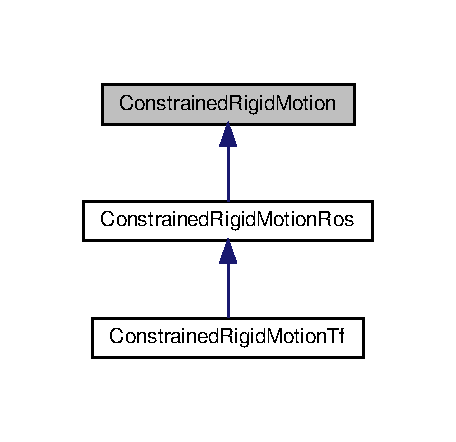
\includegraphics[width=219pt]{db/d32/classConstrainedRigidMotion__inherit__graph}
\end{center}
\end{figure}
\subsection*{Public Member Functions}
\begin{DoxyCompactItemize}
\item 
\hyperlink{group__RigidMotion_gaa85deb237e7407287829b6596997b210}{Constrained\+Rigid\+Motion} ()
\begin{DoxyCompactList}\small\item\em Construct a new \hyperlink{classConstrainedRigidMotion}{Constrained\+Rigid\+Motion} object. \end{DoxyCompactList}\item 
\hyperlink{group__RigidMotion_ga603d9727e46dc49dcf22b24870d15779}{Constrained\+Rigid\+Motion} (Eigen\+::\+Vector3d reference)
\begin{DoxyCompactList}\small\item\em Construct a new \hyperlink{classConstrainedRigidMotion}{Constrained\+Rigid\+Motion} object with given refrence vector. \end{DoxyCompactList}\item 
void \hyperlink{group__RigidMotion_ga80649fcba3aed41550ba463f405d051b}{update\+Input\+State} (Eigen\+::\+Vector3d state, Eigen\+::\+Vector3d d\+\_\+state, double time)
\begin{DoxyCompactList}\small\item\em Update procedure for the motion states. \end{DoxyCompactList}\item 
Eigen\+::\+Vector3d \hyperlink{group__RigidMotion_ga59bdced4bb2e565bc39312e5328507ef}{get\+Diff\+State} ()
\begin{DoxyCompactList}\small\item\em Get the Velocities of the destination. \end{DoxyCompactList}\item 
Eigen\+::\+Vector3d \hyperlink{group__RigidMotion_gabde902d2f91035cd5054a33dab4acc48}{get\+State} ()
\begin{DoxyCompactList}\small\item\em Get the State of destination. \end{DoxyCompactList}\item 
void \hyperlink{group__RigidMotion_gac71f6e395c1d63f54cfb837b5526236b}{set\+Reference} (Eigen\+::\+Vector3d ref)
\begin{DoxyCompactList}\small\item\em Set the reference from source to destination. \end{DoxyCompactList}\item 
void \hyperlink{group__RigidMotion_ga70771b8bb17cff0ffceadae49eab9f8e}{set\+Velocity\+Thresh} (double thresh)
\begin{DoxyCompactList}\small\item\em Set the Velocity Threshold that specifies when to calc atan2 to given value. \end{DoxyCompactList}\end{DoxyCompactItemize}
\subsection*{Static Public Member Functions}
\begin{DoxyCompactItemize}
\item 
static Eigen\+::\+Matrix3d \hyperlink{group__RigidMotion_gad4fb6e13815454559ec7e52b291489af}{create\+Diff\+Drive\+Locking} ()
\begin{DoxyCompactList}\small\item\em Create a differential drive locking matrix. \end{DoxyCompactList}\end{DoxyCompactItemize}


The documentation for this class was generated from the following files\+:\begin{DoxyCompactItemize}
\item 
include/multi\+\_\+robot\+\_\+controller/rigid\+\_\+motion/constrained\+\_\+rigid\+\_\+motion.\+h\item 
src/rigid\+\_\+motion/constrained\+\_\+rigid\+\_\+motion.\+cpp\end{DoxyCompactItemize}

\hypertarget{classConstrainedRigidMotionRos}{}\section{Constrained\+Rigid\+Motion\+Ros Class Reference}
\label{classConstrainedRigidMotionRos}\index{Constrained\+Rigid\+Motion\+Ros@{Constrained\+Rigid\+Motion\+Ros}}


Inheritance diagram for Constrained\+Rigid\+Motion\+Ros\+:\nopagebreak
\begin{figure}[H]
\begin{center}
\leavevmode
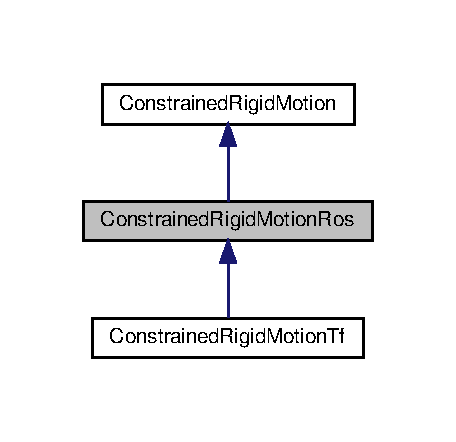
\includegraphics[width=219pt]{d4/d50/classConstrainedRigidMotionRos__inherit__graph}
\end{center}
\end{figure}


Collaboration diagram for Constrained\+Rigid\+Motion\+Ros\+:\nopagebreak
\begin{figure}[H]
\begin{center}
\leavevmode
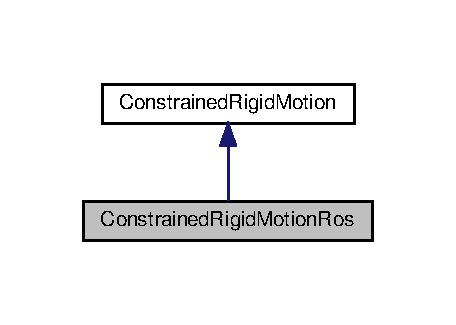
\includegraphics[width=219pt]{df/dc6/classConstrainedRigidMotionRos__coll__graph}
\end{center}
\end{figure}
\subsection*{Additional Inherited Members}


The documentation for this class was generated from the following files\+:\begin{DoxyCompactItemize}
\item 
include/multi\+\_\+robot\+\_\+controller/rigid\+\_\+motion/constrained\+\_\+rigid\+\_\+motion\+\_\+ros.\+h\item 
src/rigid\+\_\+motion/constrained\+\_\+rigid\+\_\+motion\+\_\+ros.\+cpp\end{DoxyCompactItemize}

\hypertarget{classConstrainedRigidMotionTf}{}\section{Constrained\+Rigid\+Motion\+Tf Class Reference}
\label{classConstrainedRigidMotionTf}\index{Constrained\+Rigid\+Motion\+Tf@{Constrained\+Rigid\+Motion\+Tf}}


Inheritance diagram for Constrained\+Rigid\+Motion\+Tf\+:\nopagebreak
\begin{figure}[H]
\begin{center}
\leavevmode
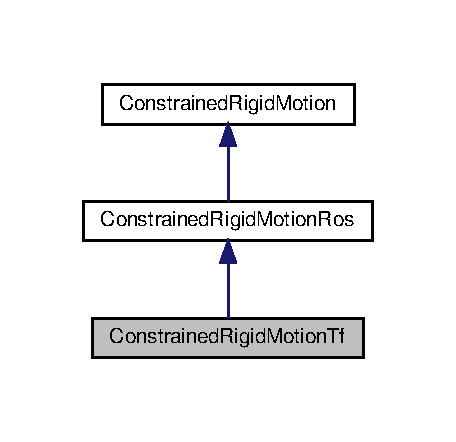
\includegraphics[width=219pt]{d2/d01/classConstrainedRigidMotionTf__inherit__graph}
\end{center}
\end{figure}


Collaboration diagram for Constrained\+Rigid\+Motion\+Tf\+:\nopagebreak
\begin{figure}[H]
\begin{center}
\leavevmode
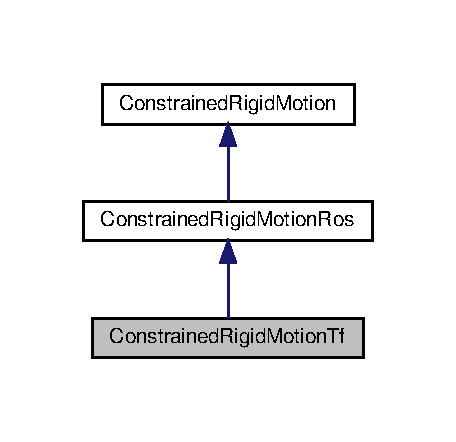
\includegraphics[width=219pt]{dc/ddf/classConstrainedRigidMotionTf__coll__graph}
\end{center}
\end{figure}
\subsection*{Public Member Functions}
\begin{DoxyCompactItemize}
\item 
void {\bfseries update\+Input\+State} (tf\+::\+Pose pose, tf\+::\+Vector3 lin\+\_\+vel, tf\+::\+Vector3 ang\+\_\+vel, double time)
\end{DoxyCompactItemize}
\subsection*{Additional Inherited Members}


The documentation for this class was generated from the following files\+:\begin{DoxyCompactItemize}
\item 
include/multi\+\_\+robot\+\_\+controller/rigid\+\_\+motion/constrained\+\_\+rigid\+\_\+motion\+\_\+tf.\+h\item 
src/rigid\+\_\+motion/constrained\+\_\+rigid\+\_\+motion\+\_\+tf.\+cpp\end{DoxyCompactItemize}

\hypertarget{classController}{}\section{Controller Class Reference}
\label{classController}\index{Controller@{Controller}}


Class for controlling a formation of multiple mobile robots.  




{\ttfamily \#include $<$controller.\+h$>$}



Inheritance diagram for Controller\+:\nopagebreak
\begin{figure}[H]
\begin{center}
\leavevmode
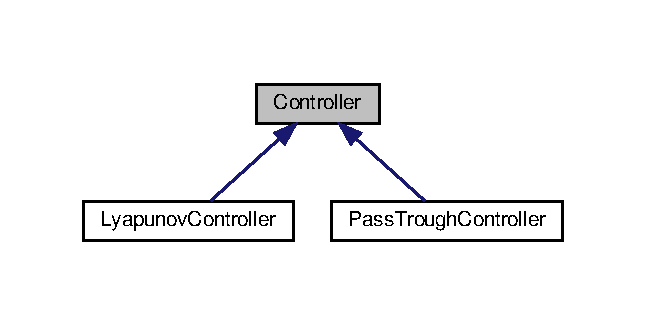
\includegraphics[width=310pt]{dc/d30/classController__inherit__graph}
\end{center}
\end{figure}


Collaboration diagram for Controller\+:\nopagebreak
\begin{figure}[H]
\begin{center}
\leavevmode
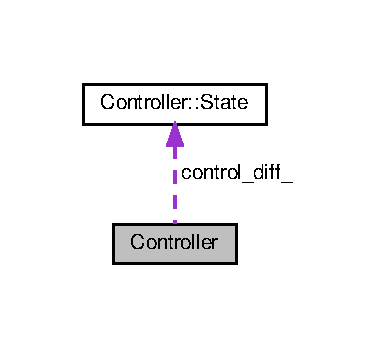
\includegraphics[width=181pt]{dd/d93/classController__coll__graph}
\end{center}
\end{figure}
\subsection*{Classes}
\begin{DoxyCompactItemize}
\item 
struct \hyperlink{structController_1_1ControlVector}{Control\+Vector}
\begin{DoxyCompactList}\small\item\em Defines the controllers output. \end{DoxyCompactList}\item 
struct \hyperlink{structController_1_1State}{State}
\begin{DoxyCompactList}\small\item\em Defines the state representations within the \hyperlink{classController}{Controller}. \end{DoxyCompactList}\end{DoxyCompactItemize}
\subsection*{Public Member Functions}
\begin{DoxyCompactItemize}
\item 
\mbox{\Hypertarget{classController_a95c56822d667e94b031451729ce069a9}\label{classController_a95c56822d667e94b031451729ce069a9}} 
\hyperlink{classController_a95c56822d667e94b031451729ce069a9}{Controller} ()
\begin{DoxyCompactList}\small\item\em Construct a new \hyperlink{classController}{Controller} object. \end{DoxyCompactList}\item 
\hyperlink{classController_a7341f9092e1977cdd2a1492c4422c019}{Controller} (ros\+::\+Node\+Handle \&nh)
\begin{DoxyCompactList}\small\item\em Construct a new \hyperlink{classController}{Controller} object with given Nodehandle. \end{DoxyCompactList}\item 
\mbox{\Hypertarget{classController_a0ab87934c4f7a266cfdb86e0f36bc1b5}\label{classController_a0ab87934c4f7a266cfdb86e0f36bc1b5}} 
\hyperlink{classController_a0ab87934c4f7a266cfdb86e0f36bc1b5}{$\sim$\+Controller} ()
\begin{DoxyCompactList}\small\item\em Destroy the \hyperlink{classController}{Controller} object. \end{DoxyCompactList}\end{DoxyCompactItemize}
\subsection*{Protected Member Functions}
\begin{DoxyCompactItemize}
\item 
virtual \hyperlink{structController_1_1ControlVector}{Control\+Vector} \hyperlink{classController_a190a3955517e39310a4b715a883cbe02}{calc\+Control} (\hyperlink{structController_1_1State}{State} current\+\_\+state, \hyperlink{structController_1_1State}{State} target\+\_\+state)=0
\begin{DoxyCompactList}\small\item\em Control law fucntion. Determines the control vector by a given current and target state. Is implemented in derived Classes. \end{DoxyCompactList}\item 
\mbox{\Hypertarget{classController_a95ac558f7a8d570ba4f0ba12182de8c5}\label{classController_a95ac558f7a8d570ba4f0ba12182de8c5}} 
virtual void \hyperlink{classController_a95ac558f7a8d570ba4f0ba12182de8c5}{publish\+Meta\+Data} ()
\begin{DoxyCompactList}\small\item\em Publishes the meta data of the controller. Thes are e.\+g. the current and target states and the control differences. \end{DoxyCompactList}\end{DoxyCompactItemize}
\subsection*{Protected Attributes}
\begin{DoxyCompactItemize}
\item 
\mbox{\Hypertarget{classController_aeb648bc7d97b36f1dcba956fa5aaeec6}\label{classController_aeb648bc7d97b36f1dcba956fa5aaeec6}} 
ros\+::\+Publisher {\bfseries meta\+\_\+}
\item 
\mbox{\Hypertarget{classController_a454701a403066ee2b8c24bd61268655e}\label{classController_a454701a403066ee2b8c24bd61268655e}} 
\hyperlink{structController_1_1State}{State} {\bfseries control\+\_\+diff\+\_\+}
\end{DoxyCompactItemize}


\subsection{Detailed Description}
Objects of this class contain the following ros parameter\+:

\tabulinesep=1mm
\begin{longtabu} spread 0pt [c]{*{2}{|X[-1]}|}
\hline
\rowcolor{\tableheadbgcolor}\textbf{ Ros-\/\+Parameter }&\textbf{ Description  }\\\cline{1-2}
\endfirsthead
\hline
\endfoot
\hline
\rowcolor{\tableheadbgcolor}\textbf{ Ros-\/\+Parameter }&\textbf{ Description  }\\\cline{1-2}
\endhead
$\sim$target/input\+\_\+type&Type of the target state topic. \\\cline{1-2}
$\sim$current/input\+\_\+type&Type of the current state topic. \\\cline{1-2}
$\sim$rate &Rate the controller is spinning with. \\\cline{1-2}
$\sim$topic\+\_\+output &Name of the output topic. \\\cline{1-2}
\end{longtabu}


\subsection{Constructor \& Destructor Documentation}
\mbox{\Hypertarget{classController_a7341f9092e1977cdd2a1492c4422c019}\label{classController_a7341f9092e1977cdd2a1492c4422c019}} 
\index{Controller@{Controller}!Controller@{Controller}}
\index{Controller@{Controller}!Controller@{Controller}}
\subsubsection{\texorpdfstring{Controller()}{Controller()}}
{\footnotesize\ttfamily Controller\+::\+Controller (\begin{DoxyParamCaption}\item[{ros\+::\+Node\+Handle \&}]{nh }\end{DoxyParamCaption})}


\begin{DoxyParams}{Parameters}
{\em nh} & Nodehandle for resolving topics \\
\hline
\end{DoxyParams}


\subsection{Member Function Documentation}
\mbox{\Hypertarget{classController_a190a3955517e39310a4b715a883cbe02}\label{classController_a190a3955517e39310a4b715a883cbe02}} 
\index{Controller@{Controller}!calc\+Control@{calc\+Control}}
\index{calc\+Control@{calc\+Control}!Controller@{Controller}}
\subsubsection{\texorpdfstring{calc\+Control()}{calcControl()}}
{\footnotesize\ttfamily virtual \hyperlink{structController_1_1ControlVector}{Control\+Vector} Controller\+::calc\+Control (\begin{DoxyParamCaption}\item[{\hyperlink{structController_1_1State}{State}}]{current\+\_\+state,  }\item[{\hyperlink{structController_1_1State}{State}}]{target\+\_\+state }\end{DoxyParamCaption})\hspace{0.3cm}{\ttfamily [protected]}, {\ttfamily [pure virtual]}}


\begin{DoxyParams}{Parameters}
{\em current\+\_\+state} & Current state of the controlled robot. \\
\hline
{\em target\+\_\+state} & \hyperlink{structController_1_1State}{State} of the mobile robot to be reached. \\
\hline
\end{DoxyParams}
\begin{DoxyReturn}{Returns}
\hyperlink{structController_1_1ControlVector}{Control\+Vector} Commands to gain the target state from current state 
\end{DoxyReturn}


The documentation for this class was generated from the following files\+:\begin{DoxyCompactItemize}
\item 
include/multi\+\_\+robot\+\_\+controller/controller/controller.\+h\item 
src/controller/controller.\+cpp\end{DoxyCompactItemize}

\hypertarget{structController_1_1ControlVector}{}\section{Controller\+:\+:Control\+Vector Struct Reference}
\label{structController_1_1ControlVector}\index{Controller\+::\+Control\+Vector@{Controller\+::\+Control\+Vector}}
\subsection*{Public Member Functions}
\begin{DoxyCompactItemize}
\item 
\mbox{\Hypertarget{structController_1_1ControlVector_abf98db4ce95ac636bb5ac950b6b820b3}\label{structController_1_1ControlVector_abf98db4ce95ac636bb5ac950b6b820b3}} 
\hyperlink{structController_1_1ControlVector_abf98db4ce95ac636bb5ac950b6b820b3}{Control\+Vector} ()
\begin{DoxyCompactList}\small\item\em Construct a new Control Vector object with default parameters. \end{DoxyCompactList}\item 
\mbox{\Hypertarget{structController_1_1ControlVector_a547dd5c56a7be54acb7c44f7fdf52c57}\label{structController_1_1ControlVector_a547dd5c56a7be54acb7c44f7fdf52c57}} 
{\bfseries Control\+Vector} (double \hyperlink{structController_1_1ControlVector_af8d8ff93ddf343a13a35bba355d39976}{v}, double \hyperlink{structController_1_1ControlVector_ad5963169c4ea0c021cb923191aef7ed3}{omega})
\end{DoxyCompactItemize}
\subsection*{Public Attributes}
\begin{DoxyCompactItemize}
\item 
\mbox{\Hypertarget{structController_1_1ControlVector_af8d8ff93ddf343a13a35bba355d39976}\label{structController_1_1ControlVector_af8d8ff93ddf343a13a35bba355d39976}} 
double \hyperlink{structController_1_1ControlVector_af8d8ff93ddf343a13a35bba355d39976}{v}
\begin{DoxyCompactList}\small\item\em Linear velocity. \end{DoxyCompactList}\item 
\mbox{\Hypertarget{structController_1_1ControlVector_ad5963169c4ea0c021cb923191aef7ed3}\label{structController_1_1ControlVector_ad5963169c4ea0c021cb923191aef7ed3}} 
double \hyperlink{structController_1_1ControlVector_ad5963169c4ea0c021cb923191aef7ed3}{omega}
\begin{DoxyCompactList}\small\item\em Angular velocity. \end{DoxyCompactList}\end{DoxyCompactItemize}


The documentation for this struct was generated from the following file\+:\begin{DoxyCompactItemize}
\item 
include/multi\+\_\+robot\+\_\+controller/controller/controller.\+h\end{DoxyCompactItemize}

\hypertarget{classInputAllocException}{}\section{Input\+Alloc\+Exception Class Reference}
\label{classInputAllocException}\index{Input\+Alloc\+Exception@{Input\+Alloc\+Exception}}


Inheritance diagram for Input\+Alloc\+Exception\+:\nopagebreak
\begin{figure}[H]
\begin{center}
\leavevmode
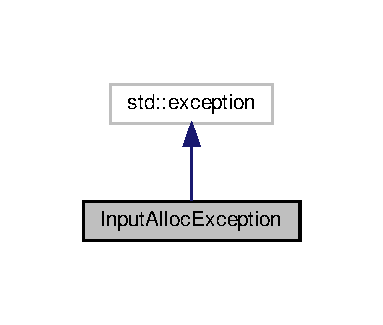
\includegraphics[width=184pt]{d8/d37/classInputAllocException__inherit__graph}
\end{center}
\end{figure}


Collaboration diagram for Input\+Alloc\+Exception\+:\nopagebreak
\begin{figure}[H]
\begin{center}
\leavevmode
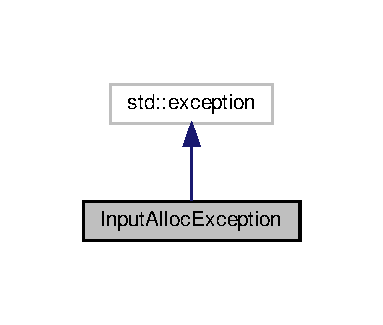
\includegraphics[width=184pt]{d5/d7d/classInputAllocException__coll__graph}
\end{center}
\end{figure}
\subsection*{Public Member Functions}
\begin{DoxyCompactItemize}
\item 
const char $\ast$ {\bfseries what} () const  throw ()
\end{DoxyCompactItemize}


The documentation for this class was generated from the following file\+:\begin{DoxyCompactItemize}
\item 
include/multi\+\_\+robot\+\_\+controller/input\+\_\+alloc\+\_\+exception.\+hpp\end{DoxyCompactItemize}

\hypertarget{classInputBase}{}\section{Input\+Base Class Reference}
\label{classInputBase}\index{Input\+Base@{Input\+Base}}


Inheritance diagram for Input\+Base\+:\nopagebreak
\begin{figure}[H]
\begin{center}
\leavevmode
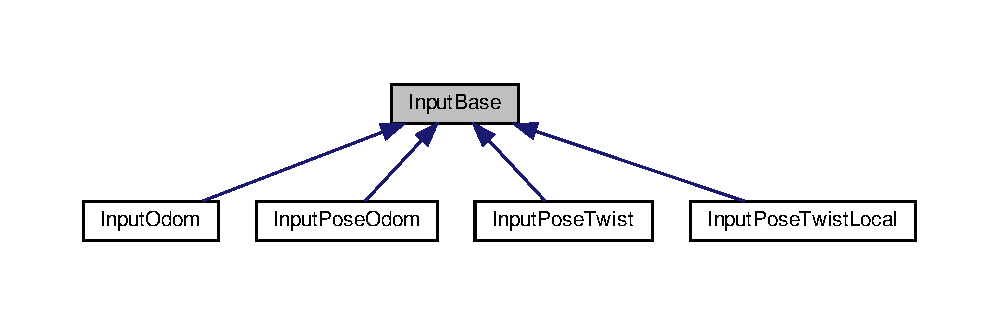
\includegraphics[width=350pt]{d8/d2a/classInputBase__inherit__graph}
\end{center}
\end{figure}
\subsection*{Public Member Functions}
\begin{DoxyCompactItemize}
\item 
{\bfseries Input\+Base} (ros\+::\+Node\+Handle \&nh)
\item 
tf\+::\+Pose {\bfseries get\+Pose} ()
\item 
tf\+::\+Vector3 {\bfseries get\+Lin\+Vel} ()
\item 
tf\+::\+Vector3 {\bfseries get\+Ang\+Vel} ()
\item 
ros\+::\+Time {\bfseries get\+Time} ()
\end{DoxyCompactItemize}
\subsection*{Protected Member Functions}
\begin{DoxyCompactItemize}
\item 
void {\bfseries check\+Values} ()
\end{DoxyCompactItemize}
\subsection*{Protected Attributes}
\begin{DoxyCompactItemize}
\item 
ros\+::\+Node\+Handle {\bfseries nh\+\_\+}
\item 
tf\+::\+Pose {\bfseries pose\+\_\+}
\item 
tf\+::\+Vector3 {\bfseries lin\+\_\+vel\+\_\+}
\item 
tf\+::\+Vector3 {\bfseries ang\+\_\+vel\+\_\+}
\item 
ros\+::\+Time {\bfseries time\+\_\+}
\end{DoxyCompactItemize}


The documentation for this class was generated from the following file\+:\begin{DoxyCompactItemize}
\item 
include/multi\+\_\+robot\+\_\+controller/input/input\+\_\+base.\+hpp\end{DoxyCompactItemize}

\hypertarget{classInputOdom}{}\section{Input\+Odom Class Reference}
\label{classInputOdom}\index{Input\+Odom@{Input\+Odom}}


Inheritance diagram for Input\+Odom\+:\nopagebreak
\begin{figure}[H]
\begin{center}
\leavevmode
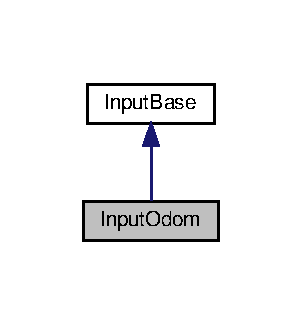
\includegraphics[width=145pt]{d6/dba/classInputOdom__inherit__graph}
\end{center}
\end{figure}


Collaboration diagram for Input\+Odom\+:\nopagebreak
\begin{figure}[H]
\begin{center}
\leavevmode
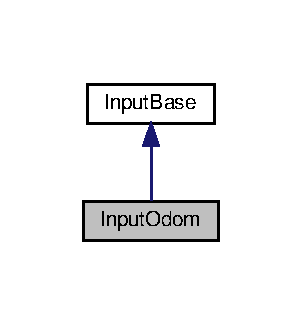
\includegraphics[width=145pt]{d5/dc5/classInputOdom__coll__graph}
\end{center}
\end{figure}
\subsection*{Public Member Functions}
\begin{DoxyCompactItemize}
\item 
{\bfseries Input\+Odom} (ros\+::\+Node\+Handle \&nh, std\+::string topic\+\_\+name)
\item 
{\bfseries Input\+Odom} (ros\+::\+Node\+Handle \&nh)
\item 
{\bfseries Input\+Odom} (ros\+::\+Node\+Handle \&nh, ros\+::\+Node\+Handle \&param\+\_\+nh)
\end{DoxyCompactItemize}
\subsection*{Additional Inherited Members}


The documentation for this class was generated from the following file\+:\begin{DoxyCompactItemize}
\item 
include/multi\+\_\+robot\+\_\+controller/input/input\+\_\+odom.\+hpp\end{DoxyCompactItemize}

\hypertarget{classInputPoseOdom}{}\section{Input\+Pose\+Odom Class Reference}
\label{classInputPoseOdom}\index{Input\+Pose\+Odom@{Input\+Pose\+Odom}}


Inheritance diagram for Input\+Pose\+Odom\+:\nopagebreak
\begin{figure}[H]
\begin{center}
\leavevmode
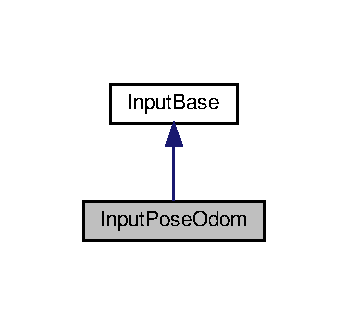
\includegraphics[width=167pt]{d3/dea/classInputPoseOdom__inherit__graph}
\end{center}
\end{figure}


Collaboration diagram for Input\+Pose\+Odom\+:\nopagebreak
\begin{figure}[H]
\begin{center}
\leavevmode
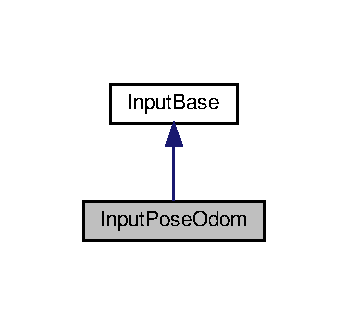
\includegraphics[width=167pt]{dd/d6d/classInputPoseOdom__coll__graph}
\end{center}
\end{figure}
\subsection*{Public Member Functions}
\begin{DoxyCompactItemize}
\item 
{\bfseries Input\+Pose\+Odom} (ros\+::\+Node\+Handle \&nh, std\+::string topic\+\_\+name\+\_\+pose, std\+::string topic\+\_\+name\+\_\+odom)
\item 
{\bfseries Input\+Pose\+Odom} (ros\+::\+Node\+Handle \&nh)
\item 
{\bfseries Input\+Pose\+Odom} (ros\+::\+Node\+Handle \&nh, ros\+::\+Node\+Handle \&nh\+\_\+param)
\end{DoxyCompactItemize}
\subsection*{Additional Inherited Members}


The documentation for this class was generated from the following file\+:\begin{DoxyCompactItemize}
\item 
include/multi\+\_\+robot\+\_\+controller/input/input\+\_\+pose\+\_\+odom.\+hpp\end{DoxyCompactItemize}

\hypertarget{classInputPoseTwist}{}\section{Input\+Pose\+Twist Class Reference}
\label{classInputPoseTwist}\index{Input\+Pose\+Twist@{Input\+Pose\+Twist}}


Inheritance diagram for Input\+Pose\+Twist\+:\nopagebreak
\begin{figure}[H]
\begin{center}
\leavevmode
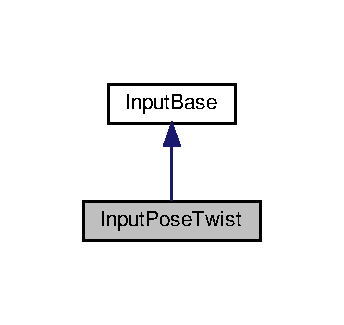
\includegraphics[width=165pt]{d7/d11/classInputPoseTwist__inherit__graph}
\end{center}
\end{figure}


Collaboration diagram for Input\+Pose\+Twist\+:\nopagebreak
\begin{figure}[H]
\begin{center}
\leavevmode
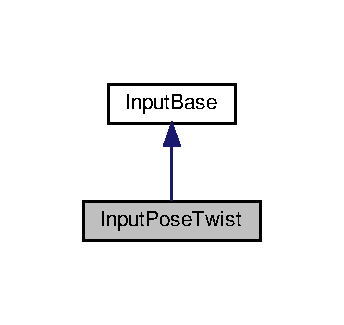
\includegraphics[width=165pt]{d6/d3a/classInputPoseTwist__coll__graph}
\end{center}
\end{figure}
\subsection*{Public Member Functions}
\begin{DoxyCompactItemize}
\item 
{\bfseries Input\+Pose\+Twist} (ros\+::\+Node\+Handle \&nh, std\+::string topic\+\_\+name\+\_\+pose, std\+::string topic\+\_\+name\+\_\+twist)
\item 
{\bfseries Input\+Pose\+Twist} (ros\+::\+Node\+Handle \&nh)
\item 
{\bfseries Input\+Pose\+Twist} (ros\+::\+Node\+Handle \&nh, ros\+::\+Node\+Handle \&nh\+\_\+param)
\end{DoxyCompactItemize}
\subsection*{Additional Inherited Members}


The documentation for this class was generated from the following file\+:\begin{DoxyCompactItemize}
\item 
include/multi\+\_\+robot\+\_\+controller/input/input\+\_\+pose\+\_\+twist.\+hpp\end{DoxyCompactItemize}

\hypertarget{classLyapunovController}{}\section{Lyapunov\+Controller Class Reference}
\label{classLyapunovController}\index{Lyapunov\+Controller@{Lyapunov\+Controller}}


Inheritance diagram for Lyapunov\+Controller\+:\nopagebreak
\begin{figure}[H]
\begin{center}
\leavevmode
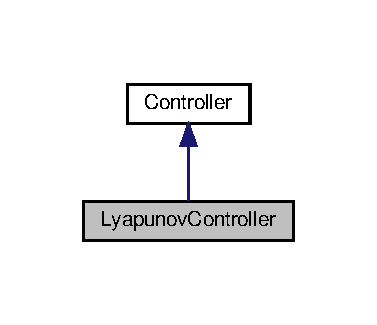
\includegraphics[width=181pt]{d9/d75/classLyapunovController__inherit__graph}
\end{center}
\end{figure}


Collaboration diagram for Lyapunov\+Controller\+:\nopagebreak
\begin{figure}[H]
\begin{center}
\leavevmode
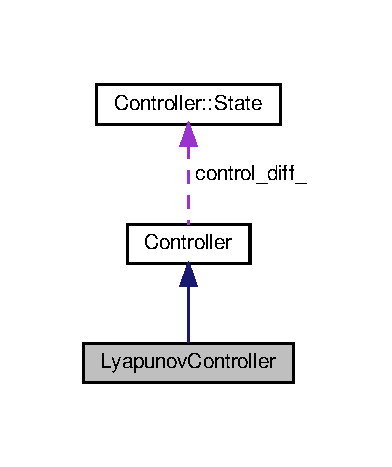
\includegraphics[width=181pt]{de/de2/classLyapunovController__coll__graph}
\end{center}
\end{figure}
\subsection*{Classes}
\begin{DoxyCompactItemize}
\item 
struct \hyperlink{structLyapunovController_1_1LyapunovParameter}{Lyapunov\+Parameter}
\begin{DoxyCompactList}\small\item\em Holds the necessary parameters for the control law. \end{DoxyCompactList}\end{DoxyCompactItemize}
\subsection*{Public Member Functions}
\begin{DoxyCompactItemize}
\item 
\hyperlink{classLyapunovController_a3b17565509b8e085861a85146738766f}{Lyapunov\+Controller} (ros\+::\+Node\+Handle \&nh, \hyperlink{structLyapunovController_1_1LyapunovParameter}{Lyapunov\+Parameter} parameterset)
\begin{DoxyCompactList}\small\item\em Construct a new Lyapunov \hyperlink{classController}{Controller} object. \end{DoxyCompactList}\item 
\hyperlink{classLyapunovController_a2812acc6b131e59ac0fc9b0633038999}{Lyapunov\+Controller} (ros\+::\+Node\+Handle \&nh)
\begin{DoxyCompactList}\small\item\em Construct a new Lyapunov \hyperlink{classController}{Controller} object and automatically load parameters from the ros parameter server. \end{DoxyCompactList}\end{DoxyCompactItemize}
\subsection*{Additional Inherited Members}


\subsection{Constructor \& Destructor Documentation}
\mbox{\Hypertarget{classLyapunovController_a3b17565509b8e085861a85146738766f}\label{classLyapunovController_a3b17565509b8e085861a85146738766f}} 
\index{Lyapunov\+Controller@{Lyapunov\+Controller}!Lyapunov\+Controller@{Lyapunov\+Controller}}
\index{Lyapunov\+Controller@{Lyapunov\+Controller}!Lyapunov\+Controller@{Lyapunov\+Controller}}
\subsubsection{\texorpdfstring{Lyapunov\+Controller()}{LyapunovController()}\hspace{0.1cm}{\footnotesize\ttfamily [1/2]}}
{\footnotesize\ttfamily Lyapunov\+Controller\+::\+Lyapunov\+Controller (\begin{DoxyParamCaption}\item[{ros\+::\+Node\+Handle \&}]{nh,  }\item[{\hyperlink{structLyapunovController_1_1LyapunovParameter}{Lyapunov\+Parameter}}]{parameterset }\end{DoxyParamCaption})}



Construct a new Lyapunov \hyperlink{classController}{Controller} object. 


\begin{DoxyParams}{Parameters}
{\em nh} & Nodehandle the controller is determining topic namespaces with \\
\hline
{\em parameterset} & Set of \hyperlink{structLyapunovController_1_1LyapunovParameter}{Lyapunov\+Parameter} for calculations \\
\hline
\end{DoxyParams}
\mbox{\Hypertarget{classLyapunovController_a2812acc6b131e59ac0fc9b0633038999}\label{classLyapunovController_a2812acc6b131e59ac0fc9b0633038999}} 
\index{Lyapunov\+Controller@{Lyapunov\+Controller}!Lyapunov\+Controller@{Lyapunov\+Controller}}
\index{Lyapunov\+Controller@{Lyapunov\+Controller}!Lyapunov\+Controller@{Lyapunov\+Controller}}
\subsubsection{\texorpdfstring{Lyapunov\+Controller()}{LyapunovController()}\hspace{0.1cm}{\footnotesize\ttfamily [2/2]}}
{\footnotesize\ttfamily Lyapunov\+Controller\+::\+Lyapunov\+Controller (\begin{DoxyParamCaption}\item[{ros\+::\+Node\+Handle \&}]{nh }\end{DoxyParamCaption})}



Construct a new Lyapunov \hyperlink{classController}{Controller} object and automatically load parameters from the ros parameter server. 


\begin{DoxyParams}{Parameters}
{\em nh} & Nodehandle the controller is determining topic namespaces with \\
\hline
\end{DoxyParams}


The documentation for this class was generated from the following files\+:\begin{DoxyCompactItemize}
\item 
include/multi\+\_\+robot\+\_\+controller/controller/lyapunov\+\_\+controller.\+h\item 
src/controller/lyapunov\+\_\+controller.\+cpp\end{DoxyCompactItemize}

\hypertarget{structLyapunovController_1_1LyapunovParameter}{}\section{Lyapunov\+Controller\+:\+:Lyapunov\+Parameter Struct Reference}
\label{structLyapunovController_1_1LyapunovParameter}\index{Lyapunov\+Controller\+::\+Lyapunov\+Parameter@{Lyapunov\+Controller\+::\+Lyapunov\+Parameter}}


Holds the necessary parameters for the control law.  




{\ttfamily \#include $<$lyapunov\+\_\+controller.\+h$>$}

\subsection*{Public Member Functions}
\begin{DoxyCompactItemize}
\item 
\mbox{\Hypertarget{structLyapunovController_1_1LyapunovParameter_afc872afae50a2b135bbae2914a7fa8c2}\label{structLyapunovController_1_1LyapunovParameter_afc872afae50a2b135bbae2914a7fa8c2}} 
\hyperlink{structLyapunovController_1_1LyapunovParameter_afc872afae50a2b135bbae2914a7fa8c2}{Lyapunov\+Parameter} (float \hyperlink{structLyapunovController_1_1LyapunovParameter_af45ecc57706f7d6b9d1fcdf2fd355fc2}{kx}=0.\+0, float \hyperlink{structLyapunovController_1_1LyapunovParameter_afcdfaafefdbafdc6cca6b2db8a45fe3a}{ky}=0.\+0, float \hyperlink{structLyapunovController_1_1LyapunovParameter_a823275a2d5ddd96019b3d69ea327c95c}{kphi}=0.\+0)
\begin{DoxyCompactList}\small\item\em Construct a new Lyapunov Parameter object with default Parameter. \end{DoxyCompactList}\item 
\hyperlink{structLyapunovController_1_1LyapunovParameter_adb9af92d34ab58d439388000eab5deeb}{Lyapunov\+Parameter} (std\+::vector$<$ float $>$ param)
\begin{DoxyCompactList}\small\item\em Construct a new Lyapunov Parameter object with given parameters by vector. \end{DoxyCompactList}\end{DoxyCompactItemize}
\subsection*{Public Attributes}
\begin{DoxyCompactItemize}
\item 
\mbox{\Hypertarget{structLyapunovController_1_1LyapunovParameter_af45ecc57706f7d6b9d1fcdf2fd355fc2}\label{structLyapunovController_1_1LyapunovParameter_af45ecc57706f7d6b9d1fcdf2fd355fc2}} 
float \hyperlink{structLyapunovController_1_1LyapunovParameter_af45ecc57706f7d6b9d1fcdf2fd355fc2}{kx}
\begin{DoxyCompactList}\small\item\em Control gain in x-\/direction. \end{DoxyCompactList}\item 
\mbox{\Hypertarget{structLyapunovController_1_1LyapunovParameter_afcdfaafefdbafdc6cca6b2db8a45fe3a}\label{structLyapunovController_1_1LyapunovParameter_afcdfaafefdbafdc6cca6b2db8a45fe3a}} 
float \hyperlink{structLyapunovController_1_1LyapunovParameter_afcdfaafefdbafdc6cca6b2db8a45fe3a}{ky}
\begin{DoxyCompactList}\small\item\em Control gain in y-\/direction. \end{DoxyCompactList}\item 
\mbox{\Hypertarget{structLyapunovController_1_1LyapunovParameter_a823275a2d5ddd96019b3d69ea327c95c}\label{structLyapunovController_1_1LyapunovParameter_a823275a2d5ddd96019b3d69ea327c95c}} 
float \hyperlink{structLyapunovController_1_1LyapunovParameter_a823275a2d5ddd96019b3d69ea327c95c}{kphi}
\begin{DoxyCompactList}\small\item\em Control gain in theta-\/direction. \end{DoxyCompactList}\end{DoxyCompactItemize}


\subsection{Constructor \& Destructor Documentation}
\mbox{\Hypertarget{structLyapunovController_1_1LyapunovParameter_adb9af92d34ab58d439388000eab5deeb}\label{structLyapunovController_1_1LyapunovParameter_adb9af92d34ab58d439388000eab5deeb}} 
\index{Lyapunov\+Controller\+::\+Lyapunov\+Parameter@{Lyapunov\+Controller\+::\+Lyapunov\+Parameter}!Lyapunov\+Parameter@{Lyapunov\+Parameter}}
\index{Lyapunov\+Parameter@{Lyapunov\+Parameter}!Lyapunov\+Controller\+::\+Lyapunov\+Parameter@{Lyapunov\+Controller\+::\+Lyapunov\+Parameter}}
\subsubsection{\texorpdfstring{Lyapunov\+Parameter()}{LyapunovParameter()}}
{\footnotesize\ttfamily Lyapunov\+Controller\+::\+Lyapunov\+Parameter\+::\+Lyapunov\+Parameter (\begin{DoxyParamCaption}\item[{std\+::vector$<$ float $>$}]{param }\end{DoxyParamCaption})\hspace{0.3cm}{\ttfamily [inline]}}


\begin{DoxyParams}{Parameters}
{\em param} & vector that must contain the three object parameters \\
\hline
\end{DoxyParams}


The documentation for this struct was generated from the following file\+:\begin{DoxyCompactItemize}
\item 
include/multi\+\_\+robot\+\_\+controller/controller/lyapunov\+\_\+controller.\+h\end{DoxyCompactItemize}

\hypertarget{classMsgOrientationFeedForward}{}\section{Msg\+Orientation\+Feed\+Forward$<$ T $>$ Class Template Reference}
\label{classMsgOrientationFeedForward}\index{Msg\+Orientation\+Feed\+Forward$<$ T $>$@{Msg\+Orientation\+Feed\+Forward$<$ T $>$}}


A Ros implementation of the Orientation\+Feeed\+Forward class. It contains a ros Subscriber that listens to a specific message and uses the message data as input data for the feed forward control.  




{\ttfamily \#include $<$msg\+\_\+orientation\+\_\+feed\+\_\+forward.\+h$>$}



Inheritance diagram for Msg\+Orientation\+Feed\+Forward$<$ T $>$\+:\nopagebreak
\begin{figure}[H]
\begin{center}
\leavevmode
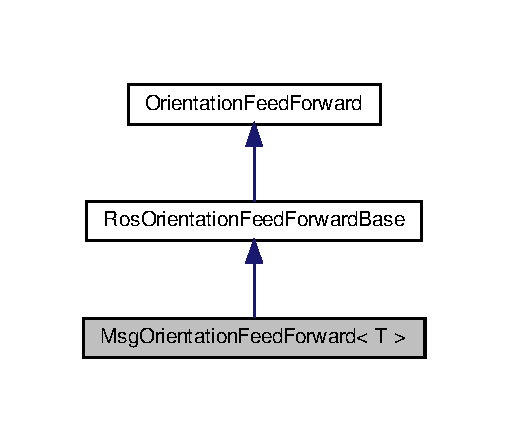
\includegraphics[width=244pt]{d0/d5b/classMsgOrientationFeedForward__inherit__graph}
\end{center}
\end{figure}


Collaboration diagram for Msg\+Orientation\+Feed\+Forward$<$ T $>$\+:\nopagebreak
\begin{figure}[H]
\begin{center}
\leavevmode
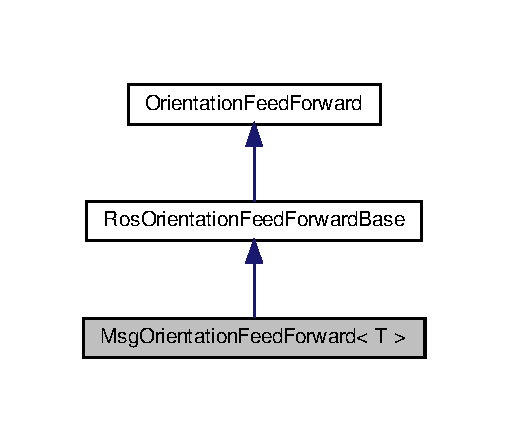
\includegraphics[width=244pt]{d2/d75/classMsgOrientationFeedForward__coll__graph}
\end{center}
\end{figure}
\subsection*{Public Member Functions}
\begin{DoxyCompactItemize}
\item 
\hyperlink{classMsgOrientationFeedForward_a487a69133c5098f14abeeeefe76306d1}{Msg\+Orientation\+Feed\+Forward} (ros\+::\+Node\+Handle \&nh, std\+::string topic)
\begin{DoxyCompactList}\small\item\em Construct a new Ros Orientation Feed Forward object. \end{DoxyCompactList}\item 
\mbox{\Hypertarget{classMsgOrientationFeedForward_ae8216c873380686eb462826e3c48cf8e}\label{classMsgOrientationFeedForward_ae8216c873380686eb462826e3c48cf8e}} 
bool {\bfseries init} () override
\end{DoxyCompactItemize}
\subsection*{Protected Member Functions}
\begin{DoxyCompactItemize}
\item 
\mbox{\Hypertarget{classMsgOrientationFeedForward_a78a74196a620861ae943af2d6d50c8af}\label{classMsgOrientationFeedForward_a78a74196a620861ae943af2d6d50c8af}} 
void {\bfseries update} (const ros\+::\+Timer\+Event \&) override
\end{DoxyCompactItemize}
\subsection*{Additional Inherited Members}


\subsection{Detailed Description}
\subsubsection*{template$<$class T$>$\newline
class Msg\+Orientation\+Feed\+Forward$<$ T $>$}


\begin{DoxyTemplParams}{Template Parameters}
{\em T} & Message type the subcriber is listeneing to. A convert\+Msg fucntion has to be implemented for it. \\
\hline
\end{DoxyTemplParams}


\subsection{Constructor \& Destructor Documentation}
\mbox{\Hypertarget{classMsgOrientationFeedForward_a487a69133c5098f14abeeeefe76306d1}\label{classMsgOrientationFeedForward_a487a69133c5098f14abeeeefe76306d1}} 
\index{Msg\+Orientation\+Feed\+Forward@{Msg\+Orientation\+Feed\+Forward}!Msg\+Orientation\+Feed\+Forward@{Msg\+Orientation\+Feed\+Forward}}
\index{Msg\+Orientation\+Feed\+Forward@{Msg\+Orientation\+Feed\+Forward}!Msg\+Orientation\+Feed\+Forward@{Msg\+Orientation\+Feed\+Forward}}
\subsubsection{\texorpdfstring{Msg\+Orientation\+Feed\+Forward()}{MsgOrientationFeedForward()}}
{\footnotesize\ttfamily template$<$class T $>$ \\
\hyperlink{classMsgOrientationFeedForward}{Msg\+Orientation\+Feed\+Forward}$<$ T $>$\+::\hyperlink{classMsgOrientationFeedForward}{Msg\+Orientation\+Feed\+Forward} (\begin{DoxyParamCaption}\item[{ros\+::\+Node\+Handle \&}]{nh,  }\item[{std\+::string}]{topic }\end{DoxyParamCaption})}


\begin{DoxyParams}{Parameters}
{\em nh} & Nodehandle for namespace handling \\
\hline
{\em topic} & Topic name that should be used as input source \\
\hline
\end{DoxyParams}


The documentation for this class was generated from the following files\+:\begin{DoxyCompactItemize}
\item 
include/multi\+\_\+robot\+\_\+controller/feed\+\_\+forward/msg\+\_\+orientation\+\_\+feed\+\_\+forward.\+h\item 
src/feed\+\_\+forward/msg\+\_\+orientation\+\_\+feed\+\_\+forward.\+cpp\end{DoxyCompactItemize}

\hypertarget{classNecessaryParamException}{}\section{Necessary\+Param\+Exception Class Reference}
\label{classNecessaryParamException}\index{Necessary\+Param\+Exception@{Necessary\+Param\+Exception}}


Inheritance diagram for Necessary\+Param\+Exception\+:\nopagebreak
\begin{figure}[H]
\begin{center}
\leavevmode
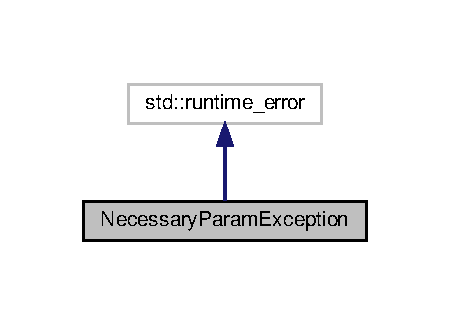
\includegraphics[width=216pt]{da/da3/classNecessaryParamException__inherit__graph}
\end{center}
\end{figure}


Collaboration diagram for Necessary\+Param\+Exception\+:\nopagebreak
\begin{figure}[H]
\begin{center}
\leavevmode
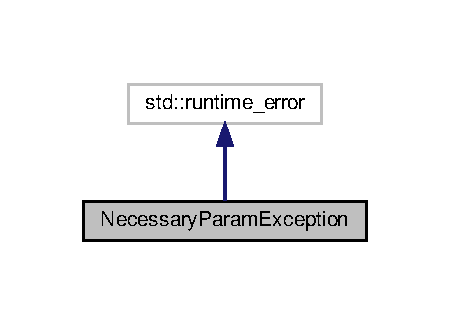
\includegraphics[width=216pt]{db/d93/classNecessaryParamException__coll__graph}
\end{center}
\end{figure}
\subsection*{Public Member Functions}
\begin{DoxyCompactItemize}
\item 
{\bfseries Necessary\+Param\+Exception} (std\+::string param\+\_\+name\+\_\+resolved)
\end{DoxyCompactItemize}


The documentation for this class was generated from the following file\+:\begin{DoxyCompactItemize}
\item 
include/multi\+\_\+robot\+\_\+controller/necessary\+\_\+param\+\_\+exeption.\+hpp\end{DoxyCompactItemize}

\hypertarget{classOrientationFeedForward}{}\section{Orientation\+Feed\+Forward Class Reference}
\label{classOrientationFeedForward}\index{Orientation\+Feed\+Forward@{Orientation\+Feed\+Forward}}


A Orientation feed forward class. It uses a given orientation and calculates a robot arm pose that compansates the motion by the change of orientation (null space motion).  




{\ttfamily \#include $<$orientation\+\_\+feed\+\_\+forward.\+h$>$}



Inheritance diagram for Orientation\+Feed\+Forward\+:\nopagebreak
\begin{figure}[H]
\begin{center}
\leavevmode
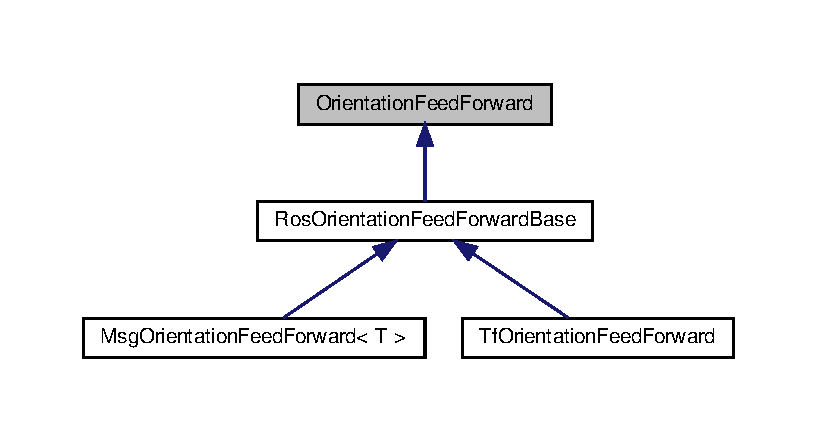
\includegraphics[width=350pt]{dd/d46/classOrientationFeedForward__inherit__graph}
\end{center}
\end{figure}
\subsection*{Public Types}
\begin{DoxyCompactItemize}
\item 
\mbox{\Hypertarget{classOrientationFeedForward_a45f6220dd29a9df06f62eeed86189101}\label{classOrientationFeedForward_a45f6220dd29a9df06f62eeed86189101}} 
typedef Eigen\+::\+Matrix$<$ double, 3, 1 $>$ {\bfseries Position}
\item 
\mbox{\Hypertarget{classOrientationFeedForward_a329654d4c6d79679903a76c624330f99}\label{classOrientationFeedForward_a329654d4c6d79679903a76c624330f99}} 
typedef Eigen\+::\+Quaterniond {\bfseries Orientation}
\item 
\mbox{\Hypertarget{classOrientationFeedForward_a68247ebc7099747e21cbd56d4dbc405a}\label{classOrientationFeedForward_a68247ebc7099747e21cbd56d4dbc405a}} 
typedef Eigen\+::\+Matrix$<$ double, 7, 1 $>$ {\bfseries Pose}
\end{DoxyCompactItemize}
\subsection*{Public Member Functions}
\begin{DoxyCompactItemize}
\item 
\mbox{\Hypertarget{classOrientationFeedForward_aad82bda1b9fa824e321a6c8afad84973}\label{classOrientationFeedForward_aad82bda1b9fa824e321a6c8afad84973}} 
\hyperlink{classOrientationFeedForward_aad82bda1b9fa824e321a6c8afad84973}{Orientation\+Feed\+Forward} ()
\begin{DoxyCompactList}\small\item\em Construct a new Orientation Feed Forward object. \end{DoxyCompactList}\item 
\hyperlink{classOrientationFeedForward_a0ae1aba3b3e0abf84828a9db008b6f69}{Orientation\+Feed\+Forward} (Position pos\+\_\+offf, Orientation ori\+\_\+off)
\begin{DoxyCompactList}\small\item\em Construct a new Orientation Feed Forward object. \end{DoxyCompactList}\item 
void \hyperlink{classOrientationFeedForward_aa7d8913f8f9d90e913b478d9adc5ff20}{update\+Orientation} (double angle)
\begin{DoxyCompactList}\small\item\em Updates the current Orientation of the mobile base that has to be feed forwarded. \end{DoxyCompactList}\item 
void \hyperlink{classOrientationFeedForward_aed8f826976135c0cd55408a652993828}{update\+Orientation} (Orientation ori)
\begin{DoxyCompactList}\small\item\em Updates the current Orientation of the mobile base that has to be feed forwarded. \end{DoxyCompactList}\item 
Pose \hyperlink{classOrientationFeedForward_ad31fce2cdf39cbf375457b9aa7ca2219}{get\+Pose} ()
\begin{DoxyCompactList}\small\item\em Get the Pose object for motion control. \end{DoxyCompactList}\item 
void \hyperlink{classOrientationFeedForward_adc105d9a1fe00d6a79fcf38447202709}{set\+Offset} (Position pos\+\_\+off, Orientation ori\+\_\+off)
\begin{DoxyCompactList}\small\item\em Set the Offset object. \end{DoxyCompactList}\item 
void \hyperlink{classOrientationFeedForward_adbd1691b1e930752818624d065acbf1c}{set\+Offset} (Pose pose)
\begin{DoxyCompactList}\small\item\em Set the Offset object. \end{DoxyCompactList}\item 
void \hyperlink{classOrientationFeedForward_a5f69dfd449972707d2ccd07e20fd2c5b}{set\+Desired\+Pose} (Pose pose)
\begin{DoxyCompactList}\small\item\em Set the Desired Pose that has to be hold in mobile base frame. \end{DoxyCompactList}\item 
void \hyperlink{classOrientationFeedForward_ad419aebf0df88282ca6c1dc24adbadb2}{set\+Desired\+Pose} (Position position, Orientation orientation)
\begin{DoxyCompactList}\small\item\em Set the Desired Pose object. \end{DoxyCompactList}\end{DoxyCompactItemize}


\subsection{Constructor \& Destructor Documentation}
\mbox{\Hypertarget{classOrientationFeedForward_a0ae1aba3b3e0abf84828a9db008b6f69}\label{classOrientationFeedForward_a0ae1aba3b3e0abf84828a9db008b6f69}} 
\index{Orientation\+Feed\+Forward@{Orientation\+Feed\+Forward}!Orientation\+Feed\+Forward@{Orientation\+Feed\+Forward}}
\index{Orientation\+Feed\+Forward@{Orientation\+Feed\+Forward}!Orientation\+Feed\+Forward@{Orientation\+Feed\+Forward}}
\subsubsection{\texorpdfstring{Orientation\+Feed\+Forward()}{OrientationFeedForward()}}
{\footnotesize\ttfamily Orientation\+Feed\+Forward\+::\+Orientation\+Feed\+Forward (\begin{DoxyParamCaption}\item[{Position}]{pos\+\_\+offf,  }\item[{Orientation}]{ori\+\_\+off }\end{DoxyParamCaption})}


\begin{DoxyParams}{Parameters}
{\em ori\+\_\+off} & The Orientation offset the Robot base has with respect to the mobile base frame \\
\hline
{\em pos\+\_\+offf} & The Position offset the Robot base has with respect to the mobile base frame \\
\hline
\end{DoxyParams}


\subsection{Member Function Documentation}
\mbox{\Hypertarget{classOrientationFeedForward_ad31fce2cdf39cbf375457b9aa7ca2219}\label{classOrientationFeedForward_ad31fce2cdf39cbf375457b9aa7ca2219}} 
\index{Orientation\+Feed\+Forward@{Orientation\+Feed\+Forward}!get\+Pose@{get\+Pose}}
\index{get\+Pose@{get\+Pose}!Orientation\+Feed\+Forward@{Orientation\+Feed\+Forward}}
\subsubsection{\texorpdfstring{get\+Pose()}{getPose()}}
{\footnotesize\ttfamily Orientation\+Feed\+Forward\+::\+Pose Orientation\+Feed\+Forward\+::get\+Pose (\begin{DoxyParamCaption}{ }\end{DoxyParamCaption})}

\begin{DoxyReturn}{Returns}
Pose in robot base frame wich can be forwarded to the robot motion control 
\end{DoxyReturn}
\mbox{\Hypertarget{classOrientationFeedForward_a5f69dfd449972707d2ccd07e20fd2c5b}\label{classOrientationFeedForward_a5f69dfd449972707d2ccd07e20fd2c5b}} 
\index{Orientation\+Feed\+Forward@{Orientation\+Feed\+Forward}!set\+Desired\+Pose@{set\+Desired\+Pose}}
\index{set\+Desired\+Pose@{set\+Desired\+Pose}!Orientation\+Feed\+Forward@{Orientation\+Feed\+Forward}}
\subsubsection{\texorpdfstring{set\+Desired\+Pose()}{setDesiredPose()}\hspace{0.1cm}{\footnotesize\ttfamily [1/2]}}
{\footnotesize\ttfamily void Orientation\+Feed\+Forward\+::set\+Desired\+Pose (\begin{DoxyParamCaption}\item[{Pose}]{pose }\end{DoxyParamCaption})}


\begin{DoxyParams}{Parameters}
{\em pose} & Desired Pose with in mobile base frame \\
\hline
\end{DoxyParams}
\mbox{\Hypertarget{classOrientationFeedForward_ad419aebf0df88282ca6c1dc24adbadb2}\label{classOrientationFeedForward_ad419aebf0df88282ca6c1dc24adbadb2}} 
\index{Orientation\+Feed\+Forward@{Orientation\+Feed\+Forward}!set\+Desired\+Pose@{set\+Desired\+Pose}}
\index{set\+Desired\+Pose@{set\+Desired\+Pose}!Orientation\+Feed\+Forward@{Orientation\+Feed\+Forward}}
\subsubsection{\texorpdfstring{set\+Desired\+Pose()}{setDesiredPose()}\hspace{0.1cm}{\footnotesize\ttfamily [2/2]}}
{\footnotesize\ttfamily void Orientation\+Feed\+Forward\+::set\+Desired\+Pose (\begin{DoxyParamCaption}\item[{Position}]{position,  }\item[{Orientation}]{orientation }\end{DoxyParamCaption})}


\begin{DoxyParams}{Parameters}
{\em position} & Position that has to be hold by the endeffektor defined in mobile base frame \\
\hline
{\em orientation} & Orientation that has to be hold by the endeffektor defined in robot base frame \\
\hline
\end{DoxyParams}
\mbox{\Hypertarget{classOrientationFeedForward_adc105d9a1fe00d6a79fcf38447202709}\label{classOrientationFeedForward_adc105d9a1fe00d6a79fcf38447202709}} 
\index{Orientation\+Feed\+Forward@{Orientation\+Feed\+Forward}!set\+Offset@{set\+Offset}}
\index{set\+Offset@{set\+Offset}!Orientation\+Feed\+Forward@{Orientation\+Feed\+Forward}}
\subsubsection{\texorpdfstring{set\+Offset()}{setOffset()}\hspace{0.1cm}{\footnotesize\ttfamily [1/2]}}
{\footnotesize\ttfamily void Orientation\+Feed\+Forward\+::set\+Offset (\begin{DoxyParamCaption}\item[{Position}]{pos\+\_\+off,  }\item[{Orientation}]{ori\+\_\+off }\end{DoxyParamCaption})}


\begin{DoxyParams}{Parameters}
{\em ori\+\_\+off} & Orientation of the Offset (from the mobile base frame and the robot frame) \\
\hline
{\em pos\+\_\+off} & Position of the Offset (from mobile base frame and the robot frame) \\
\hline
\end{DoxyParams}
\mbox{\Hypertarget{classOrientationFeedForward_adbd1691b1e930752818624d065acbf1c}\label{classOrientationFeedForward_adbd1691b1e930752818624d065acbf1c}} 
\index{Orientation\+Feed\+Forward@{Orientation\+Feed\+Forward}!set\+Offset@{set\+Offset}}
\index{set\+Offset@{set\+Offset}!Orientation\+Feed\+Forward@{Orientation\+Feed\+Forward}}
\subsubsection{\texorpdfstring{set\+Offset()}{setOffset()}\hspace{0.1cm}{\footnotesize\ttfamily [2/2]}}
{\footnotesize\ttfamily void Orientation\+Feed\+Forward\+::set\+Offset (\begin{DoxyParamCaption}\item[{Pose}]{pose }\end{DoxyParamCaption})}


\begin{DoxyParams}{Parameters}
{\em ori\+\_\+off} & Orientation of the Offset (from the mobile base frame and the robot frame) \\
\hline
{\em pos\+\_\+off} & Position of the Offset (from mobile base frame and the robot frame) \\
\hline
\end{DoxyParams}
\mbox{\Hypertarget{classOrientationFeedForward_aa7d8913f8f9d90e913b478d9adc5ff20}\label{classOrientationFeedForward_aa7d8913f8f9d90e913b478d9adc5ff20}} 
\index{Orientation\+Feed\+Forward@{Orientation\+Feed\+Forward}!update\+Orientation@{update\+Orientation}}
\index{update\+Orientation@{update\+Orientation}!Orientation\+Feed\+Forward@{Orientation\+Feed\+Forward}}
\subsubsection{\texorpdfstring{update\+Orientation()}{updateOrientation()}\hspace{0.1cm}{\footnotesize\ttfamily [1/2]}}
{\footnotesize\ttfamily void Orientation\+Feed\+Forward\+::update\+Orientation (\begin{DoxyParamCaption}\item[{double}]{angle }\end{DoxyParamCaption})}


\begin{DoxyParams}{Parameters}
{\em angle} & Angle of the Rotation around z-\/axis \\
\hline
\end{DoxyParams}
\mbox{\Hypertarget{classOrientationFeedForward_aed8f826976135c0cd55408a652993828}\label{classOrientationFeedForward_aed8f826976135c0cd55408a652993828}} 
\index{Orientation\+Feed\+Forward@{Orientation\+Feed\+Forward}!update\+Orientation@{update\+Orientation}}
\index{update\+Orientation@{update\+Orientation}!Orientation\+Feed\+Forward@{Orientation\+Feed\+Forward}}
\subsubsection{\texorpdfstring{update\+Orientation()}{updateOrientation()}\hspace{0.1cm}{\footnotesize\ttfamily [2/2]}}
{\footnotesize\ttfamily void Orientation\+Feed\+Forward\+::update\+Orientation (\begin{DoxyParamCaption}\item[{Orientation}]{ori }\end{DoxyParamCaption})}


\begin{DoxyParams}{Parameters}
{\em ori} & Quaternion of the current Orientation \\
\hline
\end{DoxyParams}


The documentation for this class was generated from the following files\+:\begin{DoxyCompactItemize}
\item 
include/multi\+\_\+robot\+\_\+controller/feed\+\_\+forward/orientation\+\_\+feed\+\_\+forward.\+h\item 
src/feed\+\_\+forward/orientation\+\_\+feed\+\_\+forward.\+cpp\end{DoxyCompactItemize}

\hypertarget{classPassTroughController}{}\section{Pass\+Trough\+Controller Class Reference}
\label{classPassTroughController}\index{Pass\+Trough\+Controller@{Pass\+Trough\+Controller}}


Inheritance diagram for Pass\+Trough\+Controller\+:\nopagebreak
\begin{figure}[H]
\begin{center}
\leavevmode
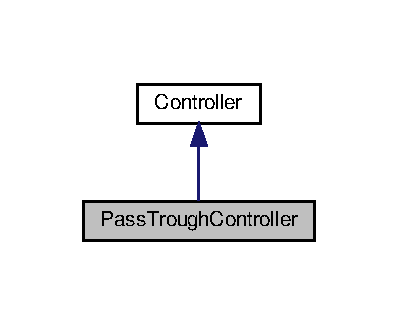
\includegraphics[width=191pt]{dc/de8/classPassTroughController__inherit__graph}
\end{center}
\end{figure}


Collaboration diagram for Pass\+Trough\+Controller\+:\nopagebreak
\begin{figure}[H]
\begin{center}
\leavevmode
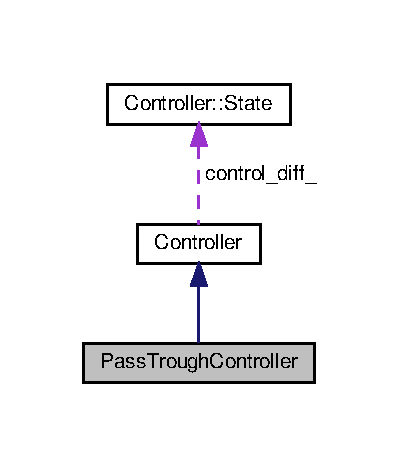
\includegraphics[width=193pt]{d5/d84/classPassTroughController__coll__graph}
\end{center}
\end{figure}
\subsection*{Public Member Functions}
\begin{DoxyCompactItemize}
\item 
\hyperlink{classPassTroughController_ab07ab9e0032dd1a46f3fd80726ce4b1f}{Pass\+Trough\+Controller} (ros\+::\+Node\+Handle nh)
\begin{DoxyCompactList}\small\item\em Construct a new Pass Trough \hyperlink{classController}{Controller} object. \end{DoxyCompactList}\end{DoxyCompactItemize}
\subsection*{Additional Inherited Members}


\subsection{Constructor \& Destructor Documentation}
\mbox{\Hypertarget{classPassTroughController_ab07ab9e0032dd1a46f3fd80726ce4b1f}\label{classPassTroughController_ab07ab9e0032dd1a46f3fd80726ce4b1f}} 
\index{Pass\+Trough\+Controller@{Pass\+Trough\+Controller}!Pass\+Trough\+Controller@{Pass\+Trough\+Controller}}
\index{Pass\+Trough\+Controller@{Pass\+Trough\+Controller}!Pass\+Trough\+Controller@{Pass\+Trough\+Controller}}
\subsubsection{\texorpdfstring{Pass\+Trough\+Controller()}{PassTroughController()}}
{\footnotesize\ttfamily Pass\+Trough\+Controller\+::\+Pass\+Trough\+Controller (\begin{DoxyParamCaption}\item[{ros\+::\+Node\+Handle}]{nh }\end{DoxyParamCaption})\hspace{0.3cm}{\ttfamily [inline]}}


\begin{DoxyParams}{Parameters}
{\em nh} & The nodehandle for topic resolving in parent class \hyperlink{classController}{Controller} \\
\hline
\end{DoxyParams}


The documentation for this class was generated from the following file\+:\begin{DoxyCompactItemize}
\item 
include/multi\+\_\+robot\+\_\+controller/controller/pass\+\_\+through\+\_\+controller.\+hpp\end{DoxyCompactItemize}

\hypertarget{classRosOrientationFeedForwardBase}{}\section{Ros\+Orientation\+Feed\+Forward\+Base Class Reference}
\label{classRosOrientationFeedForwardBase}\index{Ros\+Orientation\+Feed\+Forward\+Base@{Ros\+Orientation\+Feed\+Forward\+Base}}


A Orientation feed forward class. It implements parameter loading and initialisation for the Orientation Feed Forward class.  




{\ttfamily \#include $<$ros\+\_\+orientation\+\_\+feed\+\_\+forward\+\_\+base.\+h$>$}



Inheritance diagram for Ros\+Orientation\+Feed\+Forward\+Base\+:\nopagebreak
\begin{figure}[H]
\begin{center}
\leavevmode
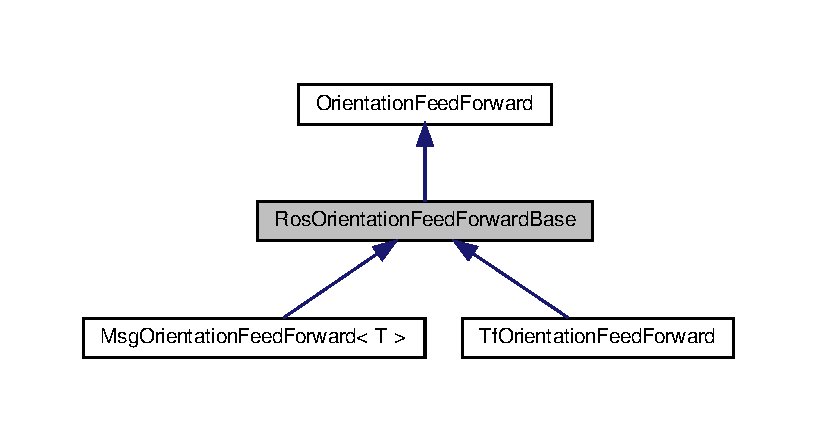
\includegraphics[width=350pt]{dc/da0/classRosOrientationFeedForwardBase__inherit__graph}
\end{center}
\end{figure}


Collaboration diagram for Ros\+Orientation\+Feed\+Forward\+Base\+:\nopagebreak
\begin{figure}[H]
\begin{center}
\leavevmode
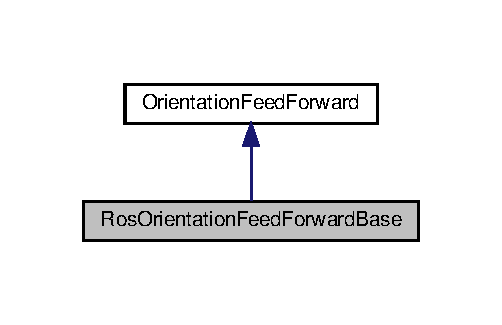
\includegraphics[width=241pt]{d6/d67/classRosOrientationFeedForwardBase__coll__graph}
\end{center}
\end{figure}
\subsection*{Public Member Functions}
\begin{DoxyCompactItemize}
\item 
\mbox{\Hypertarget{classRosOrientationFeedForwardBase_a78b33a8470ac0a61170bf3964af2b886}\label{classRosOrientationFeedForwardBase_a78b33a8470ac0a61170bf3964af2b886}} 
{\bfseries Ros\+Orientation\+Feed\+Forward\+Base} (ros\+::\+Node\+Handle \&nh)
\item 
\mbox{\Hypertarget{classRosOrientationFeedForwardBase_a272a4ee861d33ba29fa87b3d31804b60}\label{classRosOrientationFeedForwardBase_a272a4ee861d33ba29fa87b3d31804b60}} 
virtual bool {\bfseries init} ()
\end{DoxyCompactItemize}
\subsection*{Protected Member Functions}
\begin{DoxyCompactItemize}
\item 
\mbox{\Hypertarget{classRosOrientationFeedForwardBase_aae14308591e714b2b6aa01a25ee3f426}\label{classRosOrientationFeedForwardBase_aae14308591e714b2b6aa01a25ee3f426}} 
virtual void {\bfseries update} (const ros\+::\+Timer\+Event \&)=0
\end{DoxyCompactItemize}
\subsection*{Protected Attributes}
\begin{DoxyCompactItemize}
\item 
\mbox{\Hypertarget{classRosOrientationFeedForwardBase_afa860a801df238863c9f4d914b84cad2}\label{classRosOrientationFeedForwardBase_afa860a801df238863c9f4d914b84cad2}} 
ros\+::\+Node\+Handle {\bfseries nh\+\_\+}
\item 
\mbox{\Hypertarget{classRosOrientationFeedForwardBase_a056eabe353a9b022e78f00432cc0451e}\label{classRosOrientationFeedForwardBase_a056eabe353a9b022e78f00432cc0451e}} 
tf2\+\_\+ros\+::\+Transform\+Listener {\bfseries tf\+\_\+listener\+\_\+}
\item 
\mbox{\Hypertarget{classRosOrientationFeedForwardBase_af31a9db484070b9498d11c89d3c60def}\label{classRosOrientationFeedForwardBase_af31a9db484070b9498d11c89d3c60def}} 
tf2\+\_\+ros\+::\+Buffer {\bfseries tf\+\_\+buffer\+\_\+}
\item 
\mbox{\Hypertarget{classRosOrientationFeedForwardBase_a746bcb2db8165ad31cbe285be7ed9c23}\label{classRosOrientationFeedForwardBase_a746bcb2db8165ad31cbe285be7ed9c23}} 
std\+::string {\bfseries ee\+\_\+frame\+\_\+id\+\_\+}
\item 
\mbox{\Hypertarget{classRosOrientationFeedForwardBase_a71880189563e228e26ce9561e085a625}\label{classRosOrientationFeedForwardBase_a71880189563e228e26ce9561e085a625}} 
ros\+::\+Publisher {\bfseries pose\+\_\+pub\+\_\+}
\item 
\mbox{\Hypertarget{classRosOrientationFeedForwardBase_a0ac4ea0415e293dbe56fa214c1acb3fc}\label{classRosOrientationFeedForwardBase_a0ac4ea0415e293dbe56fa214c1acb3fc}} 
std\+::string {\bfseries tf\+\_\+prefix\+\_\+}
\item 
\mbox{\Hypertarget{classRosOrientationFeedForwardBase_ae3a57b29bd7a416e5dd8833d45e16754}\label{classRosOrientationFeedForwardBase_ae3a57b29bd7a416e5dd8833d45e16754}} 
ros\+::\+Service\+Server {\bfseries init\+\_\+service\+\_\+}
\end{DoxyCompactItemize}
\subsection*{Additional Inherited Members}


The documentation for this class was generated from the following files\+:\begin{DoxyCompactItemize}
\item 
include/multi\+\_\+robot\+\_\+controller/feed\+\_\+forward/ros\+\_\+orientation\+\_\+feed\+\_\+forward\+\_\+base.\+h\item 
src/feed\+\_\+forward/ros\+\_\+orientation\+\_\+feed\+\_\+forward\+\_\+base.\+cpp\end{DoxyCompactItemize}

\hypertarget{structController_1_1State}{}\section{Controller\+:\+:State Struct Reference}
\label{structController_1_1State}\index{Controller\+::\+State@{Controller\+::\+State}}


Defines the state representations within the \hyperlink{classController}{Controller}.  




{\ttfamily \#include $<$controller.\+h$>$}

\subsection*{Public Member Functions}
\begin{DoxyCompactItemize}
\item 
\mbox{\Hypertarget{structController_1_1State_abfb9cbceeaec3f0b70756e0856eff81c}\label{structController_1_1State_abfb9cbceeaec3f0b70756e0856eff81c}} 
\hyperlink{structController_1_1State_abfb9cbceeaec3f0b70756e0856eff81c}{State} ()
\begin{DoxyCompactList}\small\item\em Construct a new \hyperlink{structController_1_1State}{State} object. \end{DoxyCompactList}\item 
\hyperlink{structController_1_1State_ab75213d196a8198fec43b6737aaac530}{State} (tf\+::\+Pose pose, tf\+::\+Vector3 lin\+\_\+vel, tf\+::\+Vector3 ang\+\_\+vel)
\begin{DoxyCompactList}\small\item\em Construct a new \hyperlink{structController_1_1State}{State} object. \end{DoxyCompactList}\end{DoxyCompactItemize}
\subsection*{Public Attributes}
\begin{DoxyCompactItemize}
\item 
\mbox{\Hypertarget{structController_1_1State_a9060ab60496abb8a9658646d0f7b8cd4}\label{structController_1_1State_a9060ab60496abb8a9658646d0f7b8cd4}} 
tf\+::\+Pose {\bfseries pose}
\item 
\mbox{\Hypertarget{structController_1_1State_acaaf752c2668c1765ae9a653148df694}\label{structController_1_1State_acaaf752c2668c1765ae9a653148df694}} 
tf\+::\+Vector3 {\bfseries lin\+\_\+vel}
\item 
\mbox{\Hypertarget{structController_1_1State_a96665cd4479edd3dd44d27a1f15368dc}\label{structController_1_1State_a96665cd4479edd3dd44d27a1f15368dc}} 
tf\+::\+Vector3 {\bfseries ang\+\_\+vel}
\end{DoxyCompactItemize}


\subsection{Constructor \& Destructor Documentation}
\mbox{\Hypertarget{structController_1_1State_ab75213d196a8198fec43b6737aaac530}\label{structController_1_1State_ab75213d196a8198fec43b6737aaac530}} 
\index{Controller\+::\+State@{Controller\+::\+State}!State@{State}}
\index{State@{State}!Controller\+::\+State@{Controller\+::\+State}}
\subsubsection{\texorpdfstring{State()}{State()}}
{\footnotesize\ttfamily Controller\+::\+State\+::\+State (\begin{DoxyParamCaption}\item[{tf\+::\+Pose}]{pose,  }\item[{tf\+::\+Vector3}]{lin\+\_\+vel,  }\item[{tf\+::\+Vector3}]{ang\+\_\+vel }\end{DoxyParamCaption})}


\begin{DoxyParams}{Parameters}
{\em pose} & Pose of the mobile robot in space \\
\hline
{\em lin\+\_\+vel} & Linear velocity of the robot in space \\
\hline
{\em ang\+\_\+vel} & Angular velocity of the robot in space \\
\hline
\end{DoxyParams}


The documentation for this struct was generated from the following files\+:\begin{DoxyCompactItemize}
\item 
include/multi\+\_\+robot\+\_\+controller/controller/controller.\+h\item 
src/controller/controller.\+cpp\end{DoxyCompactItemize}

\hypertarget{classTfOrientationFeedForward}{}\section{Tf\+Orientation\+Feed\+Forward Class Reference}
\label{classTfOrientationFeedForward}\index{Tf\+Orientation\+Feed\+Forward@{Tf\+Orientation\+Feed\+Forward}}


A Tf implementation of the Orientation\+Feeed\+Forward class. It contains a tf listener that listens to a specific transformations and uses the data as input data for the feed forward control.  




{\ttfamily \#include $<$tf\+\_\+orientation\+\_\+feed\+\_\+forward.\+h$>$}



Inheritance diagram for Tf\+Orientation\+Feed\+Forward\+:\nopagebreak
\begin{figure}[H]
\begin{center}
\leavevmode
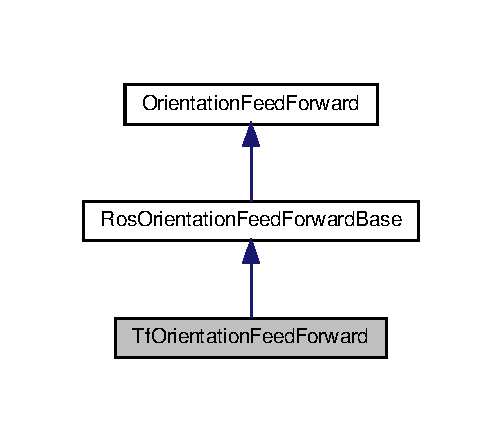
\includegraphics[width=241pt]{d3/d31/classTfOrientationFeedForward__inherit__graph}
\end{center}
\end{figure}


Collaboration diagram for Tf\+Orientation\+Feed\+Forward\+:\nopagebreak
\begin{figure}[H]
\begin{center}
\leavevmode
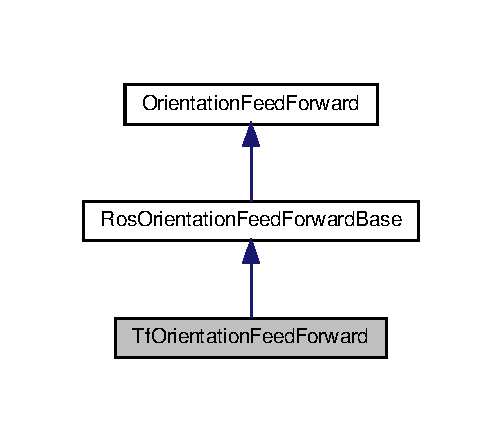
\includegraphics[width=241pt]{de/ddf/classTfOrientationFeedForward__coll__graph}
\end{center}
\end{figure}
\subsection*{Public Member Functions}
\begin{DoxyCompactItemize}
\item 
\mbox{\Hypertarget{classTfOrientationFeedForward_ac6b65030da947e765a431b5b82d600b1}\label{classTfOrientationFeedForward_ac6b65030da947e765a431b5b82d600b1}} 
{\bfseries Tf\+Orientation\+Feed\+Forward} (ros\+::\+Node\+Handle \&nh)
\item 
\mbox{\Hypertarget{classTfOrientationFeedForward_a68e54f0b974cc6aa5fab10ec5b5a18cf}\label{classTfOrientationFeedForward_a68e54f0b974cc6aa5fab10ec5b5a18cf}} 
bool {\bfseries init} () override
\end{DoxyCompactItemize}
\subsection*{Protected Member Functions}
\begin{DoxyCompactItemize}
\item 
\mbox{\Hypertarget{classTfOrientationFeedForward_aa74b9cf9be940b3d49bb6288fa88d2fa}\label{classTfOrientationFeedForward_aa74b9cf9be940b3d49bb6288fa88d2fa}} 
void {\bfseries update} (const ros\+::\+Timer\+Event \&) override
\end{DoxyCompactItemize}
\subsection*{Additional Inherited Members}


The documentation for this class was generated from the following files\+:\begin{DoxyCompactItemize}
\item 
include/multi\+\_\+robot\+\_\+controller/feed\+\_\+forward/tf\+\_\+orientation\+\_\+feed\+\_\+forward.\+h\item 
src/feed\+\_\+forward/tf\+\_\+orientation\+\_\+feed\+\_\+forward.\+cpp\end{DoxyCompactItemize}

\chapter{File Documentation}
\hypertarget{msg__conversion_8hpp}{}\section{include/multi\+\_\+robot\+\_\+controller/feed\+\_\+forward/msg\+\_\+conversion.hpp File Reference}
\label{msg__conversion_8hpp}\index{include/multi\+\_\+robot\+\_\+controller/feed\+\_\+forward/msg\+\_\+conversion.\+hpp@{include/multi\+\_\+robot\+\_\+controller/feed\+\_\+forward/msg\+\_\+conversion.\+hpp}}
{\ttfamily \#include $<$eigen3/\+Eigen/\+Dense$>$}\newline
{\ttfamily \#include $<$geometry\+\_\+msgs/\+Transform\+Stamped.\+h$>$}\newline
{\ttfamily \#include $<$geometry\+\_\+msgs/\+Transform.\+h$>$}\newline
{\ttfamily \#include $<$geometry\+\_\+msgs/\+Pose\+Stamped.\+h$>$}\newline
{\ttfamily \#include $<$geometry\+\_\+msgs/\+Pose.\+h$>$}\newline
{\ttfamily \#include $<$std\+\_\+msgs/\+Float64.\+h$>$}\newline
Include dependency graph for msg\+\_\+conversion.\+hpp\+:\nopagebreak
\begin{figure}[H]
\begin{center}
\leavevmode
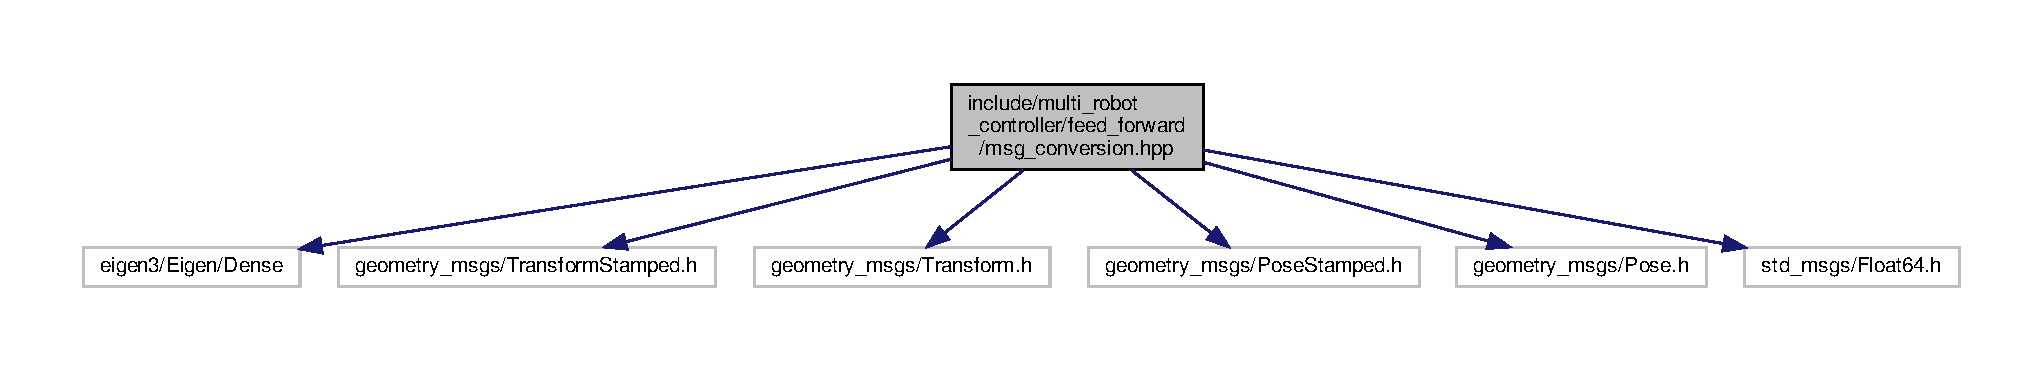
\includegraphics[width=350pt]{d9/d5a/msg__conversion_8hpp__incl}
\end{center}
\end{figure}
This graph shows which files directly or indirectly include this file\+:\nopagebreak
\begin{figure}[H]
\begin{center}
\leavevmode
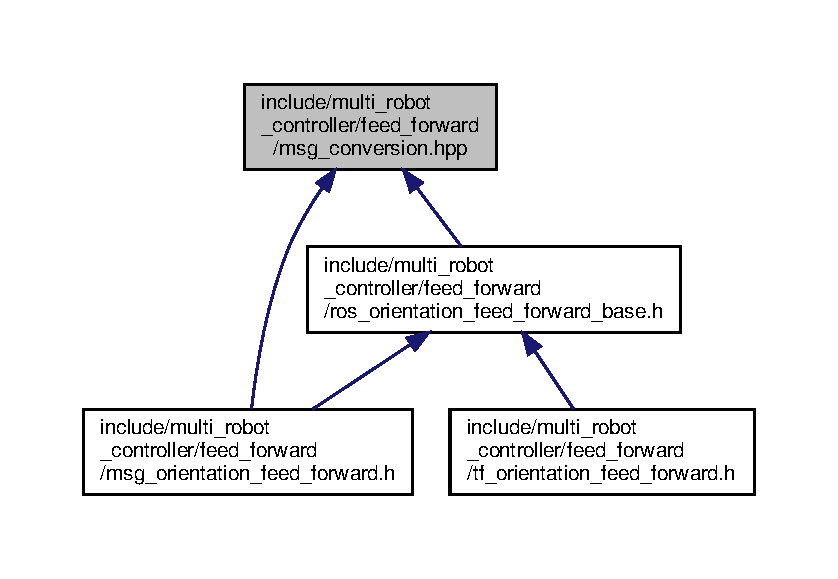
\includegraphics[width=350pt]{de/d06/msg__conversion_8hpp__dep__incl}
\end{center}
\end{figure}
\subsection*{Functions}
\begin{DoxyCompactItemize}
\item 
void \hyperlink{group__MultiRobotController_ga465b07e16106af072ed5315010fa876c}{convert\+Msg} (Eigen\+::\+Quaterniond \&quat, std\+\_\+msgs\+::\+Float64 \&msg)
\begin{DoxyCompactList}\small\item\em Convert an float64 z-\/axis angle to an eigen quaternion. \end{DoxyCompactList}\item 
void \hyperlink{group__MultiRobotController_gad42169e0be94216cd31a8a360a848155}{convert\+Msg} (Eigen\+::\+Quaterniond \&quat, geometry\+\_\+msgs\+::\+Transform \&msg)
\begin{DoxyCompactList}\small\item\em Convert Orientation of a Transform geometry message to an eigen quaternion. \end{DoxyCompactList}\item 
void \hyperlink{group__MultiRobotController_ga34987bf2293cc8aa5fac7ac60e6510ef}{convert\+Msg} (Eigen\+::\+Quaterniond \&quat, geometry\+\_\+msgs\+::\+Transform\+Stamped \&msg)
\begin{DoxyCompactList}\small\item\em Convert an Stamped\+Transform geometry message to an eigen quaternion. \end{DoxyCompactList}\item 
void \hyperlink{group__MultiRobotController_gadc07db93efb76fd809b67b74dd13b939}{convert\+Msg} (Eigen\+::\+Quaterniond \&quat, geometry\+\_\+msgs\+::\+Pose \&msg)
\begin{DoxyCompactList}\small\item\em Convert an Pose geometry message to an eigen quaternion. \end{DoxyCompactList}\item 
void \hyperlink{group__MultiRobotController_ga8257db2bb94ec53eadfe87d04b38cc0b}{convert\+Msg} (Eigen\+::\+Quaterniond \&quat, geometry\+\_\+msgs\+::\+Pose\+Stamped \&msg)
\begin{DoxyCompactList}\small\item\em Convert an stamped pose geometry message to an eigen quaternion. \end{DoxyCompactList}\item 
void \hyperlink{group__MultiRobotController_gafde5764b46f0189c2aea14ed57434708}{convert\+Msg} (Eigen\+::\+Matrix$<$ double, 7, 1 $>$ \&pose, geometry\+\_\+msgs\+::\+Pose \&msg)
\begin{DoxyCompactList}\small\item\em Convert an pose geometry message to an Eigen pose vector (x, y, z, w, x, y, z) \end{DoxyCompactList}\item 
void \hyperlink{group__MultiRobotController_ga9e842115a5f448ab0e3ba9fea93d5179}{convert\+Msg} (Eigen\+::\+Matrix$<$ double, 7, 1 $>$ \&pose, geometry\+\_\+msgs\+::\+Pose\+Stamped \&msg)
\begin{DoxyCompactList}\small\item\em Convert an stamepd pose geometry message to an Eigen pose vector (x, y, z, w, x, y, z) \end{DoxyCompactList}\item 
void \hyperlink{group__MultiRobotController_ga7beb50c98e49263d05b3b819be58d76c}{convert\+Msg} (geometry\+\_\+msgs\+::\+Pose \&msg, Eigen\+::\+Matrix$<$ double, 7, 1 $>$ \&pose)
\begin{DoxyCompactList}\small\item\em Convert an Eigen pose vector (x, y, z, w, x, y, z) to a pose geometry message. \end{DoxyCompactList}\item 
void \hyperlink{group__MultiRobotController_gaf1628de186f2d90b064f8c8b36beef53}{convert\+Msg} (geometry\+\_\+msgs\+::\+Pose\+Stamped \&msg, Eigen\+::\+Matrix$<$ double, 7, 1 $>$ \&pose)
\begin{DoxyCompactList}\small\item\em Convert an Eigen pose vector (x, y, z, w, x, y, z) to a stamepd pose geometry message. \end{DoxyCompactList}\item 
void \hyperlink{group__MultiRobotController_ga45b2bbef58d2c60ff8eeb77d221f2ab7}{convert\+Msg} (geometry\+\_\+msgs\+::\+Pose \&pose, geometry\+\_\+msgs\+::\+Transform \&transform)
\begin{DoxyCompactList}\small\item\em Convert an Eigen pose vector (x, y, z, w, x, y, z) to a transform geometry message. \end{DoxyCompactList}\item 
void \hyperlink{group__MultiRobotController_gaf99f4d3d714176ee5a3d235ffabb7d3f}{convert\+Msg} (geometry\+\_\+msgs\+::\+Pose\+Stamped \&pose, geometry\+\_\+msgs\+::\+Transform\+Stamped \&transform\+Stamped)
\begin{DoxyCompactList}\small\item\em Convert a stamped transform geometry message to a stamped pose geometry message. \end{DoxyCompactList}\item 
void \hyperlink{group__MultiRobotController_ga21e894dfe1e1216355db06776a630b09}{convert\+Msg} (Eigen\+::\+Matrix$<$ double, 7, 1 $>$ \&pose, geometry\+\_\+msgs\+::\+Transform\+Stamped \&transform\+Stamped)
\begin{DoxyCompactList}\small\item\em Convert a stamped transform geometry message to a eigen pose vector. \end{DoxyCompactList}\item 
void \hyperlink{group__MultiRobotController_ga27bedbf17c4aa6e228239ef1f1009e2b}{convert\+Msg} (geometry\+\_\+msgs\+::\+Transform \&transform, geometry\+\_\+msgs\+::\+Pose \&pose)
\begin{DoxyCompactList}\small\item\em Convert a geometry pos messag to a geometry transfomr message. \end{DoxyCompactList}\item 
void \hyperlink{group__MultiRobotController_ga83f417b8e164774e4926508549543498}{convert\+Msg} (geometry\+\_\+msgs\+::\+Transform\+Stamped \&transform, geometry\+\_\+msgs\+::\+Pose\+Stamped \&pose)
\begin{DoxyCompactList}\small\item\em Convert a geometry stamped pose message to a stamped transform geometry message. \end{DoxyCompactList}\end{DoxyCompactItemize}

%--- End generated contents ---

% Index
\backmatter
\newpage
\phantomsection
\clearemptydoublepage
\addcontentsline{toc}{chapter}{Index}
\printindex

\end{document}
